\documentclass[11pt,a4paper]{report}

% Carga del preámbulo
% ==========================================
% PREÁMBULO Y CONFIGURACIÓN DE PAQUETES
% ==========================================

\usepackage[spanish,es-tabla]{babel}
\usepackage[utf8]{inputenc}
\usepackage[margin=2.5cm]{geometry}

% Paquetes matemáticos y de física
\usepackage{amsmath,amssymb,amsfonts,amsthm}
\usepackage{physics}
\usepackage{siunitx} % Para magnitudes físicas y unidades SI

% -----------------------------------------------------------------
% DESACTIVACIÓN DEFINITIVA DEL WARNING SIUNITX + PHYSICS
% -----------------------------------------------------------------
% 1. Desactiva el mensaje de advertencia interno de LaTeX3
\ExplSyntaxOn
\msg_redirect_name:nnn { siunitx } { physics-pkg } { none }
\ExplSyntaxOff

% 2. Asigna el comando \qty a siunitx (para escribir ej: \qty{5}{\volt})
\AtBeginDocument{\RenewCommandCopy\qty\SI}
% -----------------------------------------------------------------

% Formato de listas e imágenes
\usepackage{graphicx}
\usepackage{booktabs}
\usepackage{xcolor}
\usepackage{hyperref}
\usepackage{enumitem}
\usepackage{capt-of}

% Cajas de texto personalizadas
\usepackage[most]{tcolorbox}
\tcbuselibrary{breakable}

\newcounter{problemacontador}[chapter]

% Definición de colores principales
\definecolor{maincolor}{RGB}{0, 51, 102}      % Azul oscuro académico
\definecolor{accentcolor}{RGB}{0, 128, 128}   % Verde azulado / Teal
\definecolor{boxbg}{RGB}{245, 247, 250}       % Fondo claro para cajas

% Configuración de hyperref
\hypersetup{
    colorlinks=true,
    linkcolor=maincolor,
    filecolor=magenta,      
    urlcolor=cyan,
    citecolor=accentcolor
}

% Entornos para conceptos clave y fórmulas destacadas
\newtcolorbox{concepto}[1][]{
  colback=boxbg,
  colframe=maincolor,
  fonttitle=\bfseries,
  title={#1},
  arc=2mm,
  boxrule=1pt
}

\newtcolorbox{formula}[1][]{
  colback=boxbg,
  colframe=accentcolor,
  fonttitle=\bfseries,
  title={Fórmula clave: #1},
  arc=2mm,
  boxrule=1pt
}

\newtcolorbox{problema}[1][]{
  enhanced,
  breakable,
  colback=boxbg,
  colframe=maincolor,
  fonttitle=\bfseries,
  coltitle=white,
  arc=2mm,
  boxrule=1pt,
  before upper={\refstepcounter{problemacontador}},
  title={Problema~\theproblemacontador\ifstrempty{#1}{}{: #1}},
  lower separated=true
}

% Configuración de unidades físicas
\sisetup{
  per-mode = symbol,
  separate-uncertainty = true
}

\title{\textbf{\Huge Electrónica Física}\\[0.5em] 
\Large Apuntes Teóricos y Resolución de Problemas\\[0.3em]
\small Grado en Física --- Curso 2026--2027}
\author{Apuntes de Clase}
\date{\today}

\begin{document}

\maketitle

\cleardoublepage
\tableofcontents
\cleardoublepage

% --------------------------------------------------
% INCLUSIÓN DE LOS TEMAS
% --------------------------------------------------
% !TEX root = ../main.tex
\chapter{Introducción a la Electrónica}

% ==========================================
% 1. DEFINICIÓN Y CONCEPTOS FUNDAMENTALES
% ==========================================
\section{Definición de Electrónica}

\begin{concepto}[Definición de Electrónica]
La \textbf{Electrónica} es la rama de la Física que estudia el transporte controlado de cargas eléctricas: los principios en que se basa, los dispositivos en que ocurre y las aplicaciones a que da lugar.
\end{concepto}

% ==========================================
% 2. EVOLUCIÓN HISTÓRICA DE LA ELECTRÓNICA
% ==========================================
\section{Evolución histórica de la Electrónica}

\subsection{El electrón}

El desarrollo formal de la electrónica requería la caracterización previa del portador de carga fundamental: el electrón.

\begin{itemize}
    \item \textbf{1897 --- J. J. Thomson}: Descubrimiento del electrón mediante el estudio de los rayos catódicos. Determina experimentalmente la relación entre la carga y la masa del electrón:
    \[
    \frac{q}{m_e} = \SI{1.76e11}{\coulomb\per\kilogram}
    \]
    
    \item \textbf{1909 --- R. Millikan}: Mediante el experimento de la gota de aceite, determina el valor de la carga elemental:
    \[
    q = \SI{1.6e-19}{\coulomb}
    \]
    A partir de la relación carga/masa de Thomson y el valor de $q$, se deduce la masa del electrón en reposo:
    \[
    m_e = \SI{9.1e-31}{\kilogram}
    \]
\end{itemize}

\subsection{Electrónica de vacío}

La electrónica de vacío se basa en el fenómeno de la \textbf{emisión termoiónica}, descubierto por Thomas Edison en 1880. Consiste en la liberación de electrones desde la superficie de un conductor (cátodo) al suministrarle energía térmica.

\subsubsection{Diodo de vacío (J. A. Fleming, 1904)}
Consiste en una ampolla de vidrio en la que se ha realizado el vacío y que aloja dos electrodos:
\begin{itemize}
    \item \textbf{Cátodo (filamento):} Emite electrones al calentarse por efecto Joule.
    \item \textbf{Ánodo (placa):} Recoge los electrones emitidos cuando se encuentra polarizado a un potencial positivo respecto al cátodo.
\end{itemize}

\begin{concepto}[Propiedad rectificadora]
Al polarizar el ánodo positivamente ($V_p > 0$), se establece un campo eléctrico $\vec{E}$ que acelera los electrones hacia la placa, permitiendo el paso de corriente $I_p$. Si la polarización es inversa ($V_p < 0$), los electrones son repelidos y la corriente es nula. Este comportamiento convierte al diodo de vacío en un elemento \textbf{rectificador}.
\end{concepto}

\subsubsection{Triodo de vacío (Lee de Forest, 1907)}
Introduce un tercer electrodo denominado \textbf{rejilla de control} intercalado entre el cátodo y el ánodo. Variando el potencial aplicado a la rejilla ($V_g$), se modifica de forma efectiva el campo eléctrico próximo al cátodo, permitiendo controlar grandes corrientes de placa mediante pequeñas señales de tensión. 
\begin{itemize}
    \item \textbf{Aplicaciones principales:} Amplificador de señal y detector.
\end{itemize}

\subsubsection{Tetrodo}
Para trabajar a frecuencias más altas, se introduce una segunda rejilla denominada \textbf{rejilla de pantalla} entre la rejilla de control y la placa (normalmente conectada al mismo voltaje del cátodo o a un potencial fijo).

El objetivo es reducir la capacidad parásita entre la placa y la rejilla de control. Si consideramos la placa y el cátodo como las armaduras de un condensador de placas paralelas con capacidad $C$, al colocar una placa intermedia generamos un circuito equivalente con dos condensadores en serie:
\[
\frac{1}{C_{eq}} = \frac{1}{C_1} + \frac{1}{C_2} \implies C_{eq} < C
\]
Al reducir la capacidad equivalente $C_{eq}$, disminuyen los efectos capacitivos indeseados a altas frecuencias, mejorando la respuesta del dispositivo.

\subsubsection{Pentodo}
Para solucionar el problema de la emisión secundaria de electrones que surge en el tetrodo (donde los electrones que impactan con fuerza contra la placa liberan electrones secundarios que son atraídos por la rejilla de pantalla), se añade un quinto electrodo: la \textbf{rejilla supresora}.

Esta rejilla adicional se coloca entre la rejilla de pantalla y la placa, evitándose así la pérdida de corriente en el ánodo y logrando una característica $I$-$V$ mucho más estable.

\subsubsection{Electrónica y Comunicaciones}

Las válvulas de vacío proporcionaron el impulso definitivo para la consolidación de la radio durante su denominada época dorada (décadas de 1930 y 1940). A lo largo de este periodo, surgieron tecnologías clave basadas enteramente en estos dispositivos:

\begin{itemize}
    \item \textbf{Televisión:} Aparición del iconoscopio, desarrollado por V. K. Zworykin en 1931.
    \item \textbf{Calculadora analógica:} Basada en la arquitectura del amplificador operacional.
    \item \textbf{Radar:} Desarrollado e implantado hacia 1934.
    \item \textbf{Computación digital:} Desarrollo del primer computador electrónico (ENIAC, 1945).
\end{itemize}

El contexto histórico de la Segunda Guerra Mundial impulsó de forma decisiva las aplicaciones militares de la electrónica (radiocomunicaciones móviles, sistemas de radar, etc.). Cabe destacar que todos estos avances se lograron utilizando \textbf{exclusivamente válvulas de vacío}, sin la aparición de nuevos dispositivos electrónicos fundamentales.

\subsubsection{El ENIAC y las limitaciones de la electrónica de vacío}

El \textbf{ENIAC} (\textit{Electronic Numerical Integrator And Computer}), construido en 1945 en la Universidad de Pennsylvania, se considera el primer ordenador electrónico digital de propósito general.

\begin{concepto}[Especificaciones y características del ENIAC]
\begin{itemize}
    \item \textbf{Dimensiones y componentes:} Ocupaba una superficie de unos $\SI{160}{\metre\squared}$ y albergaba aproximadamente $19\,000$ válvulas de vacío.
    \item \textbf{Capacidad de cálculo:} Realizaba cerca de $3000$ sumas y $500$ multiplicaciones por segundo.
    \item \textbf{Consumo energético:} Consumía una potencia eléctrica de $\SI{150}{\kilo\watt}$ (generando el mito urbano de que la ciudad de Filadelfia sufría apagones cuando entraba en funcionamiento).
    \item \textbf{Arquitectura de procesamiento:} Introdujo la filosofía de la electrónica moderna al ejecutar sus procesos mediante instrucciones en \textbf{lenguaje máquina}, marcando la diferencia respecto a las computadoras analógicas previas.
\end{itemize}
\end{concepto}

A pesar de utilizar lenguaje máquina, el programa (\textit{software}) no residía en una memoria volátil reescribible. Cuando se requería modificar o reprogramar el ENIAC, el proceso implicaba la manipulación mecánica y manual de unos $6000$ interruptores y la reconexión de cables, lo que demoraba su puesta en marcha durante semanas.

El desarrollo y mantenimiento del ENIAC puso de manifiesto los cuellos de botella insuperables de la tecnología basada en válvulas termoiónicas:

\begin{enumerate}
    \item \textbf{Gran tamaño físico} de las válvulas y los módulos resultantes.
    \item \textbf{Elevado consumo de potencia} y enorme disipación de calor.
    \item \textbf{Vida útil muy corta} e inestabilidad (averías continuas por fundido de filamentos)[cite: 1].
    \item \textbf{Elevado precio} de fabricación y mantenimiento.
\end{enumerate}

\subsection{El electrón y la física pre-semiconductora}
% TODO: Thomson (1897) -> q/m = 1.76e11 C/kg
% TODO: Millikan (1909) -> q = 1.6e-19 C, m_e = 9.1e-31 kg

\subsection{Electrónica de vacío}
% TODO: Emisión termoiónica (Edison, 1880)
% TODO: Diodo de vacío (Fleming, 1904) - Cátodo, Ánodo y característica rectificadora
% TODO: Triodo de vacío (Lee de Forest, 1907) - Rejilla, amplificación y detección
% TODO: Tetrodo y Pentodo (rejilla de pantalla y supresora)
% TODO: Primeras computadoras (ENIAC, 1945) y limitaciones de las válvulas (tamaño, consumo, disipación, vida útil)

\subsection{Electrónica de estado sólido}
% TODO: Avances en física de sólidos (1925 en adelante)
% TODO: Modelo Schottky (1938), Unión PN (Ohl, 1940)
% TODO: Transistor de puntas de contacto (Bardeen y Brattain, 1947)

\subsection{Electrónica integrada y Nanoelectrónica}
% TODO: Primer circuito integrado (Kilby, 1958) y tecnología planar (Noyce, 1960)
% TODO: Primer microprocesador (Intel 4004, 1971)
% TODO: Elementos discretos vs. Circuitos integrados
% TODO: Ley de Moore (1965) y escalado tecnológico (de micro a nanoescala, nodos actuales de 3-2 nm)

\subsection{Hitos y Premios Nobel de Física vinculados}
% TODO: Resumen cronológico de Premios Nobel (Thomson, Millikan, Shockley/Bardeen/Brattain, Esaki, Alferov/Kroemer/Kilby, Geim/Novoselov, Akasaki/Amano/Nakamura)

% ==========================================
% 3. CIRCUITOS ANALÓGICOS Y DIGITALES
% ==========================================
\section{Circuitos analógicos y digitales}
% TODO: Definición de señal analógica vs. señal digital
% TODO: Necesidad de conversores A/D y D/A

% ==========================================
% 4. APLICACIONES DE LA ELECTRÓNICA
% ==========================================
\section{Aplicaciones de la Electrónica}
% TODO: Telecomunicaciones, automatización/control, electrónica de potencia, medicina, domótica, etc.
% !TEX root = ../main.tex
\chapter{Propiedades Físicas de los Semiconductores}

% ==========================================
% 2.1 SEMICONDUCTORES SIMPLES Y COMPUESTOS
% ==========================================
\section{Semiconductores simples y compuestos}

Los materiales semiconductores se dividen fundamentalmente en dos categorías según su composición química:

\begin{itemize}
    \item \textbf{Semiconductores simples o elementales:} Formados por un solo tipo de átomo perteneciente al Grupo IV de la tabla periódica, principalmente el Silicio ($\text{Si}$) y el Germanio ($\text{Ge}$).
    \item \textbf{Semiconductores compuestos:} Combinación de elementos de diferentes grupos:
    \begin{itemize}
        \item \textbf{Binarios III-V:} Arseniuro de Galio ($\text{GaAs}$), Fosfuro de Indio ($\text{InP}$), Nitruro de Galio ($\text{GaN}$).
        \item \textbf{Binarios IV-IV:} Carburo de Silicio ($\text{SiC}$).
    \end{itemize}
\end{itemize}

\subsection{Clasificación de los sólidos según la ordenación atómica}

Atendiendo a la ordenación espacial de sus átomos a larga y corta distancia, clasificamos los sólidos en tres tipos fundamentales:

\begin{enumerate}
    \item \textbf{Amorfos:} No presentan un orden periódico ni a corta ni a larga distancia. Los átomos se disponen de forma desordenada.
    \item \textbf{Policristalinos:} Formados por un agregado de pequeños dominios monocristalinos (denominados \textit{granos}) orientados al azar y separados por fronteras de grano.
    \item \textbf{Monocristalinos} (\textit{Single crystals}): Presentan una red cristalina periódica y continua a lo largo de todo el volumen del material.
\end{enumerate}

\begin{concepto}[Importancia de los monocristales en Electrónica]
En la fabricación de dispositivos electrónicos se requieren materiales \textbf{monocristalinos}. La periodicidad perfecta de la red permite aplicar el teorema de Bloch y definir estructuras de \textbf{bandas de energía concretas y bien definidas}, garantizando un control preciso sobre las propiedades de transporte electrónico y óptico.
\end{concepto}

\subsection{Estructuras de red y espacio recíproco}

Las redes cristalinas de los semiconductores más relevantes se construyen a partir de variaciones de la red cúbica.

\subsubsection{Redes cúbicas básicas}
\begin{itemize}
    \item \textbf{Cúbica simple (\textit{sc}):} Átomos únicamente en los vértices del cubo.
    \item \textbf{Cúbica centrada en el cuerpo (\textit{bcc}):} Átomos en los vértices y uno adicional en el centro geométrico del cubo.
    \item \textbf{Cúbica centrada en las caras (\textit{fcc}):} Átomos en los vértices y en el centro de cada una de las 6 caras.
\end{itemize}

\subsubsection{Red recíproca y Primera Zona de Brillouin}
Para el estudio teórico de las bandas de energía y la dinámica de portadores, resulta esencial analizar el comportamiento en el \textbf{espacio recíproco} (espacio de vectores de onda $\vec{k}$):
\begin{itemize}
    \item La red directa de la mayoría de los semiconductores ($\text{Si}$, $\text{GaAs}$) es de tipo \textbf{fcc}.
    \item La red recíproca correspondiente a una red directa \textit{fcc} es una red \textbf{bcc}.
    \item La \textbf{Primera Zona de Brillouin} (construcción de Wigner-Seitz en la red recíproca) adopta la forma geométrica de un \textbf{octaedro truncado}.
\end{itemize}

\subsection{Estructura cristalina del Silicio y Arseniuro de Galio}

\subsubsection{Silicio ($\text{Si}$): Estructura de diamante}
El Silicio pertenece al Grupo IV de la tabla periódica y cristaliza en la \textbf{estructura de diamante}. Esta red se describe geométricamente como dos redes cúbicas centradas en las caras (\textit{fcc}) interpenetradas, donde la segunda red se encuentra desplazada respecto a la primera una distancia igual a un cuarto de la diagonal principal del cubo:
\[
\Delta \vec{r} = \left( \frac{a}{4}, \frac{a}{4}, \frac{a}{4} \right)
\]

Esta disposición provoca que dentro de la celda unidad de la primera red queden 4 átomos completos de la segunda red:
\begin{itemize}
    \item Cada átomo de Silicio se sitúa en el centro de un \textbf{tetraedro regular}, rodeado por 4 átomos vecinos situados en los vértices.
    \item Los 4 electrones de valencia del $\text{Si}$ se comparten con los 4 vecinos mediante \textbf{enlaces covalentes} altamente estables.
\end{itemize}

\begin{formula}[Cálculo del número de átomos por celda y densidad atómica del Silicio]
El número de átomos por celda unidad en la estructura de diamante se calcula sumando las contribuciones de las posiciones cristalográficas:
\[
N_{\text{átomos}} = \underbrace{\frac{8 \text{ vértices}}{8}}_{\text{contribución vértices}} + \underbrace{\frac{6 \text{ caras}}{2}}_{\text{contribución caras}} + \underbrace{4 \text{ interiores}}_{\text{red interpenetrada}} = 1 + 3 + 4 = 8 \text{ átomos/celda}
\]

Sabiendo que el parámetro de red (constante de arista del cubo) del Silicio es $a = \SI{5.43}{\text{\AA}} = \SI{0.543}{\nano\meter}$, la \textbf{densidad atómica} ($\rho$) resulta:
\[
\rho = \frac{N_{\text{átomos}}}{V_{\text{celda}}} = \frac{8}{a^3} = \frac{8}{(\SI{5.43e-8}{\cm})^3} \approx \SI{5e22}{\text{átomos/cm}^3}
\]
\end{formula}

\subsubsection{Arseniuro de Galio ($\text{GaAs}$): Estructura zinc-blenda}
El Arseniuro de Galio ($\text{GaAs}$) es un semiconductor compuesto III-V que cristaliza en la \textbf{estructura zinc-blenda} (o esfalerita).

\begin{itemize}
    \item Su ordenación geométrica es idéntica a la estructura de diamante del Silicio (dos redes \textit{fcc} interpenetradas desplazadas a un cuarto de la diagonal), pero con la diferencia de que los átomos están alternados:
    \begin{itemize}
        \item Una de las subredes \textit{fcc} está ocupada enteramente por átomos de Galio ($\text{Ga}$, Grupo III).
        \item La otra subred \textit{fcc} está ocupada por átomos de Arsenio ($\text{As}$, Grupo V).
    \end{itemize}
    \item Cada átomo de $\text{Ga}$ está coordinado tetraédricamente con 4 átomos de $\text{As}$ a su alrededor, y viceversa, combinando enlaces de carácter covalent e iónico parcial.
\end{itemize}

% !TEX root = ../main.tex

% ==========================================
% 2.2 BANDAS DE ENERGÍA Y DINÁMICA DE PORTADORES
% ==========================================
\section{Bandas de energía y dinámica de portadores}

Para determinar la respuesta eléctrica de un semiconductor, es imprescindible conocer la cantidad de electrones y huecos disponibles para la conducción. Dado que la distribución de estos portadores es un problema fundamentalmente energético, se requiere el estudio de la estructura de \textbf{bandas de energía} del cristal.

\subsection{Origen de las bandas de energía en semiconductores}

Tomemos como referencia el átomo de Silicio ($\text{Si}$), con número atómico $Z = 14$ y configuración electrónica $1s^2 2s^2 2p^6 3s^2 3p^2$:
\begin{itemize}
    \item \textbf{10 electrones de capas internas:} Corresponden a los niveles $n=1$ y $n=2$ ($1s, 2s, 2p$). Están fuertemente ligados al núcleo atómico y no participan en la conducción eléctrica.
    \item \textbf{4 electrones de valencia:} Pertenecen al nivel externo $n=3$ ($3s^2 3p^2$). Se encuentran débilmente ligados y son los responsables de los enlaces interatómicos y de los fenómenos de transporte.
\end{itemize}

\subsubsection{Evolución energética al formar la red cristalina}
Para un sistema aislado de $N$ átomos de Silicio separados por una distancia infinita ($r \to \infty$), existen $2N$ estados $3s$ completamente ocupados y $6N$ estados $3p$ ocupados por $2N$ electrones (disponiendo de $4N$ estados vacíos).

A medida que los átomos se aproximan para formar la red cristalina y la distancia interatómica $r$ disminuye hasta la distancia de equilibrio $r = a_0$:
\begin{enumerate}
    \item Las funciones de onda de los electrones de valencia comienzan a solaparse.
    \item Por el \textbf{principio de exclusión de Pauli}, los niveles energéticos discretos se desdoblan en bandas continuas de estados permitidos.
    \item En la posición de equilibrio $r = a_0$, los $8N$ estados de valencia iniciales se dividen equitativamente en dos bandas permitidas separadas por una \textbf{banda prohibida} (\textit{bandgap}, $E_g$):
\end{enumerate}

\begin{concepto}[Banda de Valencia y Banda de Conducción a $T = \SI{0}{\kelvin}$]
\begin{itemize}
    \item \textbf{Banda de Conducción (BC):} Banda superior formada por $4N$ estados permitidos. A $T = \SI{0}{\kelvin}$, se encuentra totalmente \textbf{vacía} (0 electrones). Su nivel de mínima energía se denota por $E_C$.
    \item \textbf{Banda de Valencia (BV):} Banda inferior formada por $4N$ estados permitidos. A $T = \SI{0}{\kelvin}$, alberga a los $4N$ electrones de valencia, por lo que se encuentra totalmente \textbf{llena}. Su nivel de máxima energía se denota por $E_V$.
    \item \textbf{Banda Prohibida ($E_g$):} Intervalo energético de anchura $E_g = E_C - E_V$ donde no existen estados cuánticos permitidos para los electrones.
\end{itemize}
\end{concepto}

\subsection{Relación con el modelo de enlaces y condición de conducción}

Desde el punto de vista del modelo de enlaces, la situación a $T = \SI{0}{\kelvin}$ se corresponde con la red monocristalina perfecta: cada átomo de silicio comparte sus 4 electrones de valencia con 4 átomos vecinos mediante enlaces covalentes estables.

\begin{concepto}[Ausencia de conducción a $T = \SI{0}{\kelvin}$]
A $T = \SI{0}{\kelvin}$ el semiconductor \textbf{no presenta conducción eléctrica} ($\sigma = 0$). Aunque el material contiene un número elevado de cargas eléctricas, una \textbf{banda completamente llena} (BV) no permite el movimiento neto de carga al no disponer de estados vacíos accesibles a los que los electrones puedan cambiar tras aplicar un campo eléctrico. Del mismo modo, una \textbf{banda completamente vacía} (BC) no conduce por ausencia total de portadores.
\end{concepto}

\subsection{Generación térmica de portadores y concepto de hueco}

Cuando la temperatura aumenta ($T > \SI{0}{\kelvin}$), la energía térmica del sistema ($E_{\text{th}} \approx k_B T$) excita la red cristalina:

\begin{itemize}
    \item \textbf{Modelo de enlaces:} El aporte térmico rompe algunos enlaces covalentes, liberando electrones que pueden moverse por el cristal. La ruptura del enlace deja una vacante o carga positiva neta en la posición atómica original.
    \item \textbf{Modelo de bandas:} Corresponde al salto de un electrón desde la Banda de Valencia ($E_V$) a la Banda de Conducción ($E_C$), superando la energía del gap $E_g$.
\end{itemize}

\begin{concepto}[El Hueco ($h^+$) como portador de carga]
La vacante dejada en la Banda de Valencia por el electrón promovido a la Banda de Conducción se comporta como una cuasipartícula con \textbf{carga positiva $+q$}, denominada \textbf{hueco}. La conducción en la BV se produce mediante el desplazamiento de electrones adyacentes que van rellenando la vacante, lo que equivale físicamente al movimiento del hueco en sentido opuesto.
\end{concepto}

\subsection{Conductividad del Silicio intrínseco a \texorpdfstring{$T = \SI{300}{\kelvin}$}{T = 300 K}}

A temperatura ambiente ($T = \SI{300}{\kelvin}$), la energía térmica disponible ($k_B T \approx \SI{0.0259}{\eV}$) es pequeña en comparación con la anchura del gap del silicio ($E_g \approx \SI{1.12}{\eV}$).

\begin{formula}[Concentración intrínseca y conductividad del Silicio]
En el Silicio intrínseco a $T = \SI{300}{\kelvin}$:
\begin{itemize}
    \item La densidad total de electrones de valencia en la BV es aproximadamente $2 \times 10^{23} \text{ electrones/cm}^3$.
    \item La energía térmica solo logra promocionar a la BC una concentración intrínseca de electrones:
    \[
    n = p = n_i \approx \SI{1e10}{\per\cm\cubed}
    \]
    \item Esto significa que solo 1 de cada $2 \times 10^{13}$ electrones de valencia se libera a la banda de conducción.
    \item Como consecuencia, la \textbf{conductividad eléctrica} del silicio intrínseco resulta extremadamente baja:
    \[
    \sigma \approx \SI{2.5e-6}{\per\ohm\per\cm}
    \]
\end{itemize}
Por lo tanto, el silicio puro a temperatura ambiente se comporta prácticamente como un \textbf{aislante eléctrico}.
\end{formula}

% ==========================================
% PROPIEDADES FORMALES Y ESTRUCTURA DE BANDAS
% ==========================================
\subsection{Cálculo formal y propiedades de las bandas de energía}

El cálculo estricto de las bandas de energía en un cristal se fundamenta en la \textbf{hipótesis adiabática} (considerar los núcleos e iones fijos) y en la \textbf{aproximación de partícula única}, donde cada electrón se mueve bajo un potencial eficaz periódico $V(\vec{r}) = V(\vec{r} + \vec{R})$.

La resolución de la ecuación de Schrödinger independiente del tiempo:
\[
\left[ -\frac{\hbar^2}{2m} \nabla^2 + V(\vec{r}) \right] \psi(\vec{r}) = \epsilon \, \psi(\vec{r})
\]
proporciona como soluciones las \textbf{funciones de Bloch}:
\[
\psi_{n,\vec{k},\sigma}(\vec{r}) = e^{i \vec{k} \cdot \vec{r}} u_{n,\vec{k},\sigma}(\vec{r}), \quad \text{con } u(\vec{r}) = u(\vec{r} + \vec{R})
\]
donde $n$ representa el índice de banda, $\vec{k}$ el vector de onda y $\sigma$ el índice de espín. La energía $\epsilon_n(\vec{k})$ presenta la periodicidad de la red recíproca, por lo que basta con determinarla en la \textbf{Primera Zona de Brillouin (1ZB)}.

Debido a la finitud del cristal, el vector de onda $\vec{k}$ está cuantizado. Para una red cúbica con $N^3$ celdas de arista $a$, las componentes se expresan como:
\[
k_x = \frac{p_x}{N} \frac{\pi}{a}, \quad \text{con } p_x = -N, -(N-1), \dots, 0, \dots, (N-1)
\]
El elevado número de estados discretos permite considerar $\vec{k}$ como un continuo con una densidad de estados en el espacio recíproco igual a $V / (8\pi^3)$.

\subsubsection{Aproximación parabólica y superficies isoenergéticas}
En las proximidades de un extremo de banda (mínimo de BC o máximo de BV) situado en $\vec{k}_0$, se realiza el desarrollo en serie de Taylor de la energía $\epsilon_n(\vec{k})$:
\[
\epsilon_n(\vec{k}) \approx \epsilon_n(\vec{k}_0) + \frac{1}{2} \sum_{i,j} \left. \frac{\partial^2 \epsilon}{\partial k_i \partial k_j} \right|_{\vec{k}_0} (k_i - k_{i0})(k_j - k_{j0})
\]
donde el término de primer orden se anula ($\nabla_{\vec{k}} \epsilon_n(\vec{k}_0) = 0$) por la condición de extremo local.

Por la simetría del cristal, siempre es posible encontrar un sistema de ejes principales donde la matriz de derivadas segundas (el tensor de masa efectiva) sea diagonal:
\[
\epsilon_n(\vec{k}) \approx \epsilon_n(\vec{k}_0) + \frac{1}{2} \sum_{i} \left. \frac{\partial^2 \epsilon}{\partial k_i^2} \right|_{\vec{k}_0} (k_i - k_{i0})^2
\]

Esta aproximación de segundo orden define \textbf{bandas parabólicas} cuyos contornos de energía constante (superficies isoenergéticas en el espacio $\vec{k}$) adoptan distintas geometrías:
\begin{itemize}
    \item \textbf{Elipsoides de revolución:} Surgen cuando dos coeficientes diagonales son iguales y uno es distinto ($m_x^* = m_y^* \neq m_z^*$).
    \item \textbf{Superficies esféricas:} Ocurren cuando los tres coeficientes son idénticos ($m_x^* = m_y^* = m_z^* = m^*$). La relación $\epsilon(\vec{k}) = \epsilon_0 \pm \frac{\hbar^2 k^2}{2m^*}$ es análoga a la de una partícula libre.
\end{itemize}

\subsection{Bandas de energía en el Silicio (Si) y Arseniuro de Galio (GaAs)}

La estructura energética de un semiconductor se representa graficando la energía $\epsilon(\vec{k})$ frente al módulo del vector de onda $|\vec{k}|$ a lo largo de direcciones cristalográficas de alta simetría de la 1ZB:
\begin{itemize}
    \item \textbf{Dirección $\Gamma - X$ ($[100]$):} Recorre desde el centro de la zona ($\Gamma$, $\vec{k}=0$) hasta el centro de las caras cuadradas. Existen 6 direcciones equivalentes.
    \item \textbf{Dirección $\Gamma - L$ ($[111]$):} Recorre desde $\Gamma$ hacia el centro de las caras hexagonales. Existen 8 direcciones equivalentes.
\end{itemize}

\subsubsection{Comparativa: Gap Directo vs. Gap Indirecto}

\begin{concepto}[Diferencia fundamental entre Silicio y GaAs]
\begin{itemize}
    \item \textbf{Silicio ($\text{Si}$ --- Gap Indirecto):} El máximo de la Banda de Valencia se sitúa en el punto $\Gamma$ ($\vec{k}=0$), pero el mínimo absoluto de la Banda de Conducción se localiza en la dirección $\Gamma-X$ ($[100]$). Para promocionar un electrón desde la BV a la BC se requiere una variación neta de momento ($\Delta \vec{k} \neq 0$), exigiendo la absorción o emisión de un \textbf{fonón}.
    \item \textbf{Arseniuro de Galio ($\text{GaAs}$ --- Gap Directo):} Tanto el máximo de la BV como el mínimo absoluto de la BC coinciden en el punto $\Gamma$ ($\vec{k}=0$). El salto de banda no requiere conservación de momento adicional ($\Delta \vec{k} \approx 0$), lo que otorga al GaAs una elevada actividad optoelectrónica.
\end{itemize}
\end{concepto}

\subsubsection{Distribución de los extremos de banda y valles equivalentes}

\begin{enumerate}
    \item \textbf{Silicio ($\text{Si}$, $E_g = \SI{1.12}{\eV}$):}
    \begin{itemize}
        \item \textbf{Banda de Conducción:} Presenta el mínimo en la dirección $\Gamma-X$ ($[100]$) a un $85\%$ de la distancia al borde de la 1ZB. Posee \textbf{6 valles equivalentes} de geometría elipsoidal orientados según los ejes $\pm k_x, \pm k_y, \pm k_z$.
        \item \textbf{Banda de Valencia:} Máximo esférico en $\Gamma$.
    \end{itemize}

    \item \textbf{Arseniuro de Galio ($\text{GaAs}$, $E_g = \SI{1.42}{\eV}$):}
    \begin{itemize}
        \item \textbf{Mínimo principal en $\Gamma$:} Es único, de geometría esférica y con una curvatura muy pronunciada, lo que se traduce en una \textbf{masa efectiva pequeña} y mayor movilidad de electrones.
        \item \textbf{Mínimos secundarios (Valles $L$ y $X$):} Existen sub-bandas superiores con mínimos locales a mayor energía:
        \begin{itemize}
            \item \textbf{Valles $L$ ($[111]$):} Situados a $\Delta E = \SI{0.31}{\eV}$ sobre el mínimo principal. Al estar en los centros de las 8 caras hexagonales en el borde de zona (compartidas por dos celdas adyacentes), el número de valles equivalentes en la 1ZB es:
            \[
            N_L = \frac{8}{2} = 4 \text{ valles equivalentes}
            \]
            \item \textbf{Valles $X$ ($[100]$):} Situados a $\Delta E = \SI{0.51}{\eV}$ sobre el mínimo principal. Al estar en las caras cuadradas compartidas, su número es:
            \[
            N_X = \frac{6}{2} = 3 \text{ valles equivalentes}
            \]
        \end{itemize}
        \item \textbf{Efecto en la masa efectiva:} Los electrones promovidos a los valles $L$ o $X$ se encuentran en regiones de menor curvatura de banda, por lo que su \textbf{masa efectiva es mayor} y se desplazan a menor velocidad.
    \end{itemize}
\end{enumerate}

% ==========================================
% DINÁMICA DEL ELECTRÓN Y CONCEPTO DE HUECO
% ==========================================
\subsection{Dinámica del electrón en la red cristalina}

En un cristal perfecto sin campos exteriores, las funciones de Bloch $\psi_{n,\vec{k}}(\vec{r}) = e^{i \vec{k} \cdot \vec{r}} u_{n,\vec{k}}(\vec{r})$ constituyen un conjunto completo de estados de energía estacionarios. %[cite: 2]

Para describir el movimiento del electrón bajo la acción de fuerzas externas débiles $\vec{F}$ (como campos eléctricos o magnéticos), se utiliza la \textbf{aproximación semiclásica}. %[cite: 2] Se construye un paquete de ondas centrado en un vector de onda $\vec{k}$, cuya velocidad de grupo coincide con la velocidad media del electrón: %[cite: 2]
\[
\langle \vec{v}_k \rangle = \frac{1}{\hbar} \vec{\nabla}_{\vec{k}} \, \varepsilon(\vec{k}) %[cite: 2]
\]

La evolución temporal del vector de onda en presencia de una fuerza externa viene dada por la ecuación del movimiento semiclásica: %[cite: 2]
\[
\hbar \frac{d\vec{k}}{dt} = \vec{F} %[cite: 2]
\]

\subsubsection{Deducción del Tensor de Masa Efectiva}

Para determinar la aceleración del electrón en el sólido, calculamos la derivada temporal de la componente $i$-ésima de la velocidad de grupo: %[cite: 2]
\[
\frac{d}{dt} \langle v_k \rangle_i = \frac{d}{dt} \left[ \frac{1}{\hbar} \frac{\partial \varepsilon}{\partial k_i} \right] %[cite: 2]
\]

Aplicando la regla de la cadena para la dependencia temporal en $\vec{k}(t)$: %[cite: 2]
\[
\frac{d}{dt} \langle v_k \rangle_i = \frac{1}{\hbar} \sum_j \frac{\partial^2 \varepsilon}{\partial k_i \partial k_j} \frac{dk_j}{dt} %[cite: 2]
\]

Sustituyendo la ecuación semiclásica $\frac{dk_j}{dt} = \frac{F_j}{\hbar}$: %[cite: 2]
\[
\frac{d}{dt} \langle v_k \rangle_i = \sum_j \left( \frac{1}{\hbar^2} \frac{\partial^2 \varepsilon}{\partial k_i \partial k_j} \right) F_j %[cite: 2]
\]

\begin{concepto}[Tensor Masa Efectiva Inversa]
Definimos las componentes del \textbf{tensor masa efectiva inversa} como: %[cite: 2]
\[
\left( \frac{1}{m^*} \right)_{i,j} = \frac{1}{\hbar^2} \frac{\partial^2 \varepsilon}{\partial k_i \partial k_j} %[cite: 2]
\]
Este tensor engloba toda la interacción interna del potencial periódico del cristal sobre el electrón. %[cite: 2] La aceleración adopta una forma análoga a la segunda ley de Newton: %[cite: 2]
\[
\frac{d}{dt} \langle \vec{v}_k \rangle = \left( \frac{1}{m^*} \right) \vec{F} %[cite: 2]
\]
\end{concepto}

\subsubsection{Masa efectiva en los extremos de banda}

Al expandir en serie de Taylor la energía en torno a un extremo de banda ($\vec{k}_0$) expresado en sus ejes principales: %[cite: 2]
\[
\varepsilon(\vec{k}) = \varepsilon(\vec{k}_0) \pm \sum_i \frac{\hbar^2 k_i^2}{2 m_{ii}^*} %[cite: 2]
\]
donde el signo positivo corresponde a un mínimo de banda (fondo de la Banda de Conducción) y el signo negativo a un máximo de banda (techo de la Banda de Valencia). %[cite: 2]

En el caso particular de \textbf{bandas esféricas}, las masas principales son iguales ($m_{xx}^* = m_{yy}^* = m_{zz}^* = m^*$), por lo que la masa efectiva se reduce a un escalar: %[cite: 2]
\begin{formula}[Relación de dispersión para bandas esféricas]
\[
\varepsilon(k) = \pm \frac{\hbar^2 k^2}{2m^*} %[cite: 2]
\]
\end{formula}

\newpage
% ==========================================
% CONCEPTO DE HUECO Y PORTADORES LIBRES
% ==========================================
\subsection{El concepto de hueco y dinámica colectiva}

En el techo de la Banda de Valencia (BV), la curvatura de la relación de dispersión es negativa ($\frac{\partial^2 \varepsilon}{\partial k^2} < 0$), lo que se traduce en una \textbf{masa efectiva negativa} ($m^* = -|m^*|$). Un electrón individual en esta región presentaría un movimiento anómalo, acelerando en sentido opuesto a la fuerza exterior aplicada. 

Para resolver esta descripción, se analiza el comportamiento eléctrico global del conjunto de electrones en una banda casi llena.

\subsubsection{Deducción formal de la densidad de corriente}

La densidad de corriente eléctrica $\vec{J}$ debida a los electrones en la Banda de Valencia equivale a la suma sobre todos los estados ocupados por cargas $q = -e$:
\[
\vec{J} = \sum_{\text{ocupados}} q \, \vec{v}_i
\]

Podemos expresar esta suma como la contribución de una banda completamente llena menos la contribución de los estados vacíos (vacantes):
\[
\vec{J} = \sum_{\text{todos}} q \, \vec{v}_j - \sum_{\text{vacíos}} q \, \vec{v}_v
\]

Por la simetría de la zona de Brillouin, a cada estado con velocidad $\vec{v}$ le corresponde otro con velocidad $-\vec{v}$, de modo que la corriente total de una banda completamente llena es nula ($\sum_{\text{todos}} q \, \vec{v}_j = 0$). Sustituyendo $q = -e$:
\[
\vec{J} = - \sum_{\text{vacíos}} (-e) \, \vec{v}_v = \sum_{\text{vacíos}} (+e) \, \vec{v}_v
\]

\begin{concepto}[Equivalencia física del hueco]
El movimiento colectivo de los electrones en la Banda de Valencia es matemáticamente equivalente al transporte de carga realizado por partículas ficticias denominadas \textbf{huecos} ($h^+$), presentes en cantidad igual a los estados vacíos, con velocidad $\vec{v}_v$ y \textbf{carga positiva} $+e = \SI{1.6e-19}{\coulomb}$.
\end{concepto}

\subsubsection{Dinámica del hueco bajo un campo eléctrico}

Al aplicar un campo eléctrico externo $\vec{E}$, la fuerza sobre un electrón en el techo de la BV con $m^* = -|m^*|$ produce la siguiente aceleración:
\[
\vec{F} = q \vec{E} = m^* \vec{a} \implies \vec{a} = \frac{-e \vec{E}}{-|m^*|} = \frac{+e \vec{E}}{|m^*|}
\]

Esta aceleración es idéntica a la que experimentaría una partícula de \textbf{carga positiva} $+e$ y \textbf{masa efectiva positiva} $|m^*|$.

\begin{formula}[Propiedades del hueco]
El hueco se define como una cuasipartícula que describe los estados vacíos en la BV con las siguientes características:
\begin{itemize}
    \item \textbf{Carga eléctrica:} $q_h = +e = \SI{1.6e-19}{\coulomb}$.
    \item \textbf{Masa efectiva:} $m_p^* = |m^*| > 0$ (positiva).
    \item \textbf{Relación de dispersión:} Responde a la misma curva $\varepsilon(\vec{k})$ que los electrones.
    \item \textbf{Escala energética:} La energía del hueco aumenta hacia abajo en el diagrama de bandas (cuanto más profundo se encuentra en la BV respecto a $E_V$).
\end{itemize}
\end{formula}

\subsection{Portadores libres en el semiconductor}

Los \textbf{portadores libres} son las cargas con libertad de movimiento a lo largo del cristal que contribuyen de forma efectiva a la conducción eléctrica. Existen únicamente dos tipos de portadores libres en un semiconductor:

\begin{enumerate}
    \item \textbf{Electrones en la Banda de Conducción ($e^-$):} Localizados en las proximidades del mínimo de la BC ($E_C$), caracterizados por masa efectiva positiva ($m_n^* > 0$) y carga negativa ($q = -e$).
    \item \textbf{Huecos en la Banda de Valencia ($h^+$):} Localizados en las proximidades del máximo de la BV ($E_V$), caracterizados por masa efectiva positiva ($m_p^* > 0$) y carga positiva ($q = +e$).
\end{enumerate}

\begin{concepto}[Portadores intrínsecos a $T > \SI{0}{\kelvin}$]
A temperatura ambiente ($T = \SI{300}{\kelvin}$), la energía térmica ($E_{\text{th}} \approx k_B T$) promociona electrones desde $E_V$ hasta $E_C$, generando pares electrón-hueco. 

Sin embargo, debido a la magnitud del gap energético ($E_g \gg k_B T$), el número de portadores libres generados térmicamente en un semiconductor puro (intrínseco) es \textbf{extremadamente reducido} (por ejemplo, $n_i \approx \SI{1e10}{\cm^{-3}}$ en el silicio frente a $\sim 10^{23} \text{ electrones/cm}^3$ de valencia).
\end{concepto}

\newpage

% ==========================================
% 2.3 SEMICONDUCTORES INTRÍNSECOS Y EXTRÍNSECOS
% ==========================================
\section{Semiconductores intrínsecos y extrínsecos}

\subsection{Semiconductores intrínsecos}

Un \textbf{semiconductor intrínseco} es aquel material cristalográficamente perfecto que está compuesto exclusivamente por los átomos propios del elemento semiconductor (por ejemplo, Silicio puro), libre de impurezas o defectos en la red.

En esta condición ideal a $T = \SI{0}{\kelvin}$, todos los electrones de valencia están fuertemente ligados a los enlaces covalentes, por lo que la Banda de Conducción está vacía y la Banda de Valencia completamente llena.

Al aumentar la temperatura ($T > \SI{0}{\kelvin}$), la energía térmica promedio de las partículas viene dada por:
\[
E_{\text{th}} = \frac{3}{2} k_B T
\]
A $T = \SI{300}{\kelvin}$, este aporte térmico equivale a $E_{\text{th}} \approx \SI{0.038}{\eV}$. Aunque esta energía es inferior a la anchura del gap ($E_g \approx \SI{1.12}{\eV}$ para el Silicio), la distribución estadística permite la ruptura de un número muy reducido de enlaces covalentes:
\begin{itemize}
    \item Los electrones ligados en los enlaces corresponden a estados en la Banda de Valencia.
    \item Al romper un enlace, el electrón liberado pasa a la Banda de Conducción.
    \item La vacante generada en el enlace constituye un hueco ($h^+$) libre en la Banda de Valencia.
\end{itemize}

\begin{formula}[Densidad intrínseca de portadores]
En un semiconductor intrínseco, los portadores se generan estrictamente por pares electrón-hueco, por lo que la concentración de electrones libres ($n$) es exactamente igual a la de huecos libres ($p$):
\[
n = p = n_i
\]
donde $n_i$ representa la \textbf{densidad intrínseca de portadores}. Para el Silicio a $T = \SI{300}{\kelvin}$:
\[
n_i \approx \SI{1e10}{\cm^{-3}}
\]
Dado que la densidad total de electrones de valencia es de aproximadamente $2 \times 10^{23} \text{ e}^-/\text{cm}^3$, la conductividad resultante ($\sigma \approx \SI{2.5e-6}{\per\ohm\per\cm}$) hace que el semiconductor intrínseco se comporte como un aislante práctico.
\end{formula}

\subsection{Semiconductores extrínsecos: El proceso de dopado}

Para aumentar la conductividad eléctrica de forma controlada y adaptar el material para aplicaciones electrónicas, se introducen impurezas de otros elementos químicos en proporciones muy pequeñas (proceso denominado \textbf{dopado}).

Según el tipo de elemento dopante introducido en la red cristalina, se distinguen dos clases de semiconductores extrínsecos:

\subsubsection{Caso 1: Impurezas donadoras y semiconductores tipo N}

Se introducen átomos del Grupo V de la tabla periódica (por ejemplo, Fósforo $\text{P}$ con número atómico $Z=15$, o Arsénico $\text{As}$) en una densidad $N_D$:
\begin{itemize}
    \item El átomo de Fósforo tiene 5 electrones de valencia. 4 de estos electrones forman enlaces covalentes con los 4 átomos de Silicio vecinos.
    \item El quinto electrón queda excedente y débilmente ligado al núcleo de la impureza mediante una atracción coulombiana apantallada.
    \item En el diagrama de bandas, este estado se representa como un nivel discreto de energía $E_d$ situado ligeramente por debajo de la Banda de Conducción ($E_C$).
\end{itemize}

\begin{concepto}[Ionización donadora y tipo N]
La energía de ionización requerida para liberar el quinto electrón es $\Delta E = E_C - E_d$. Como esta energía es del orden de unos pocos milielectronvoltios ($\approx \SI{0.045}{\eV}$ en el $\text{Si}$), la energía térmica ambiente ($E_{\text{th}}$) es suficiente para ionizar prácticamente todos los átomos donadores.

Cada impureza donadora aporta:
\begin{enumerate}
    \item Un electrón libre en la Banda de Conducción.
    \item Un ión donador positivo ($N_D^+$) fijo e inmóvil en la red cristalina.
\end{enumerate}
Dado que $n \gg p$, el material resultante se denomina \textbf{semiconductor extrínseco tipo N}, donde los electrones son los portadores mayoritarios.
\end{concepto}

\subsubsection{Caso 2: Impurezas aceptadoras y semiconductores tipo P}

Se introducen átomos del Grupo III de la tabla periódica (por ejemplo, Boro $\text{B}$ con número atómico $Z=5$, o Aluminio $\text{Al}$) en una densidad $N_A$:
\begin{itemize}
    \item El átomo de Boro dispone únicamente de 3 electrones de valencia para formar enlaces con los 4 átomos de Silicio vecinos.
    \item Se genera una vacante o defecto de enlace local débilmente ligado al átomo de Boro.
    \item En el diagrama de bandas, esta vacante discreta se sitúa en un nivel de energía $E_a$ ubicado ligeramente por encima de la Banda de Valencia ($E_V$).
\end{itemize}

\begin{concepto}[Ionización aceptadora y tipo P]
La energía de ionización necesaria para promover un electrón de la BV al nivel aceptador es $\Delta E = E_a - E_V$. Dado que esta energía es reducida ($\approx \SI{0.045}{\eV}$ en el $\text{Si}$), los electrones de la Banda de Valencia saltan fácilmente al nivel $E_a$ ocupando la vacante de la impureza.

Cada impureza aceptadora aporta:
\begin{enumerate}
    \item Un hueco libre ($h^+$) en la Banda de Valencia.
    \item Un ión aceptador negativo ($N_A^-$) fijo e inmóvil en la red cristalina.
\end{enumerate}
Dado que $p \gg n$, el material resultante se denomina \textbf{semiconductor extrínseco tipo P}, donde los huecos son los portadores mayoritarios.
\end{concepto}

\newpage

% ==========================================
% CARACTERIZACIÓN ENERGÉTICA DE LOS ESTADOS
% ==========================================
\subsection{Caracterización energética de los estados}

\subsubsection{a) Estados de Bloch}

Los estados de Bloch son el resultado directo de la periodicidad espacial del potencial cristalino. En el espacio recíproco, la densidad de estados por unidad de volumen del espacio real y del espacio recíproco es constante:
\[
g(\vec{k}) = \frac{1}{4\pi^3}
\]

Para determinar la \textbf{densidad de estados en energía} $g(\varepsilon)$ (número de estados cuánticos por unidad de energía y unidad de volumen del espacio real), se integra sobre la superficie de energía constante $S(\varepsilon)$ en el espacio $\vec{k}$:
\[
g(\varepsilon) = \frac{1}{4\pi^3} \int_{S(\varepsilon)} \frac{dS}{|\vec{\nabla}_{\vec{k}} \varepsilon|}
\]

Para el caso de bandas parabólicas con superficies isoenergéticas esféricas:
\[
\varepsilon = \varepsilon_0 \pm \frac{\hbar^2 k^2}{2m^*}
\]
donde el signo positivo ($+$) corresponde al mínimo de la Banda de Conducción ($\varepsilon_0 = E_C$) y el signo negativo ($-$) al máximo de la Banda de Valencia ($\varepsilon_0 = E_V$).

Sustituyendo el gradiente de la energía en la integral de superficie, obtenemos la expresión general:
\[
g(\varepsilon) = \frac{4\pi}{h^3} (2m^*)^{3/2} (\pm \varepsilon \mp \varepsilon_0)^{1/2}
\]

\begin{formula}[Densidades de estados en las bandas de conducción y valencia]
Aplicando esta expresión a cada una de las bandas permitidas:
\begin{itemize}
    \item \textbf{Banda de Conducción ($g_C(\varepsilon)$):}
    \[
    g_C(\varepsilon) = \frac{4\pi}{h^3} (2m_n^*)^{3/2} (\varepsilon - E_C)^{1/2}, \quad (\varepsilon \ge E_C)
    \]
    \item \textbf{Banda de Valencia ($g_V(\varepsilon)$):}
    \[
    g_V(\varepsilon) = \frac{4\pi}{h^3} (2m_p^*)^{3/2} (E_V - \varepsilon)^{1/2}, \quad (\varepsilon \le E_V)
    \]
\end{itemize}
\end{formula}

\subsubsection{b) Estados asociados a impurezas (modelo hidrogenoide)}

Al introducir una impureza sustitucional en la red (por ejemplo, el quinto electrón de valencia de una impureza donadora como el Fósforo), el electrón extra experimenta dos interacciones fundamentales:
\begin{enumerate}
    \item \textbf{Aproximación de masa efectiva:} El efecto global del potencial periódico del cristal sobre el electrón se engloba en el término cinético mediante la masa efectiva $m^*$.
    \item \textbf{Interacción Coulombiana en el medio:} La atracción electrostática entre el núcleo de la impureza (con una carga positiva neta adicional $+e$) y el electrón no ocurre en el vacío, sino en el seno del semiconductor con permitividad dieléctrica $\varepsilon_{\text{SC}} = \varepsilon_r \varepsilon_0$.
\end{enumerate}

La ecuación de Schrödinger estacionaria para este sistema adopta la forma:
\[
\left( -\frac{\hbar^2}{2m^*} \nabla^2 - \frac{e^2}{4\pi \varepsilon_{\text{SC}} r} \right) \phi(\vec{r}) = \varepsilon \, \phi(\vec{r})
\]

Esta ecuación es formalmente idéntica a la del átomo de hidrógeno, sustituyendo la masa del electrón libre $m_0$ por la masa efectiva $m^*$ y la permitividad del vacío $\varepsilon_0$ por $\varepsilon_{\text{SC}}$. Los niveles de energía resultantes que ligan el electrón al átomo de la impureza son:
\[
\varepsilon_n = - \frac{13.6}{\varepsilon_r^2} \left( \frac{m^*}{m_0} \right) \frac{1}{n^2} \quad \text{(eV)}
\]

\begin{concepto}[Origen de niveles y ocupación de los estados de impureza]
Tomando como origen de energías el fondo de la Banda de Conducción ($E_C$), la energía requerida para liberar el electrón hacia la BC es el estado fundamental $n=1$, conocido como energía de ionización $\Delta E = E_C - E_d$.

Los niveles excitados ($n > 1$) no se ocupan en la práctica. La razón física es que el núcleo del átomo de la impureza posee únicamente una carga positiva adicional; por lo tanto, una vez ocupado el estado fundamental por un electrón, la atracción electrostática queda apantallada y un segundo electrón no se verá atraído. Por ello, los estados de impureza se comportan en la práctica como un único nivel discreto ($E_d$ para donadores, $E_a$ para aceptadores).
\end{concepto}

\subsubsection{Comparativa: Estados de Bloch vs. Estados de Impurezas}

\begin{table}[h!]
\centering
\begin{tabular}{
  >{\raggedright\arraybackslash}p{0.3\textwidth}
  >{\raggedright\arraybackslash}p{0.32\textwidth}
  >{\raggedright\arraybackslash}p{0.32\textwidth}
}
\toprule
\textbf{Propiedad} & \textbf{Estados de Bloch} & \textbf{Estados de Impurezas} \\
\midrule
\textbf{Localización espacial} & No localizados espacialmente (funciones extendidas, periódicas de la red). & Localizados espacialmente (orbitales hidrogenoides en torno al átomo de impureza). \\
\addlinespace
\textbf{Distribución en energía} & Continuo de estados permitidos que forman bandas (con densidad $g(\varepsilon)$). & Niveles discretos de energía en la banda prohibida ($E_d$ o $E_a$). \\
\addlinespace
\textbf{Estadística de ocupación} & Ocupación independiente entre estados (obedecen estadística de Fermi-Dirac). & Ocupación dependiente (la ocupación de un estado bloquea la de los demás por repulsión coulombiana). \\
\bottomrule
\end{tabular}
\caption{Diferencias fundamentales entre los estados de Bloch y los estados de impurezas hidrogenoides.}
\end{table}

\newpage

% ==========================================
% ESTADÍSTICA DE OCUPACIÓN DE ESTADOS
% ==========================================
\subsection{Estadística de ocupación}
\subsubsection{a) Estados de Bloch}

Los electrones son fermiones y, por tanto, obedecen la \textbf{estadística de Fermi-Dirac}. La probabilidad de que un estado cuántico de Bloch con energía $\varepsilon$ esté ocupado por un electrón en equilibrio térmico a una temperatura $T$ viene dada por la función de distribución:
\[
f(\varepsilon) = \frac{1}{1 + \exp\left(\frac{\varepsilon - E_F}{k_B T}\right)}
\]
donde $E_F$ representa el \textbf{nivel de Fermi} y $k_B$ es la constante de Boltzmann.

\paragraph{Comportamiento con la temperatura}
\begin{itemize}
    \item \textbf{A cero absoluto ($T = \SI{0}{\kelvin}$):} La distribución se comporta como una función escalón ideal:
    \[
    f(\varepsilon) = \begin{cases} 
    1, & \text{si } \varepsilon < E_F \\ 
    0, & \text{si } \varepsilon > E_F 
    \end{cases}
    \]
    Todos los estados cuánticos con energía inferior a $E_F$ están completamente ocupados, mientras que todos los estados con energía superior a $E_F$ están totalmente vacíos.
    
    \item \textbf{A temperatura finita ($T > \SI{0}{\kelvin}$):} La agitación térmica suaviza la distribución, apareciendo una cola de ocupación para energías superiores a $E_F$. Para cualquier temperatura $T > \SI{0}{\kelvin}$, la probabilidad de ocupación en el propio nivel de Fermi es exactamente la mitad:
    \[
    f(E_F) = \frac{1}{2}
    \]
\end{itemize}

\begin{concepto}[Interpretación del Nivel de Fermi en Semiconductores]
En semiconductores intrínsecos o moderadamente dopados, el nivel de Fermi $E_F$ se localiza habitualmente dentro de la \textbf{banda prohibida} (\textit{gap}). Puesto que no existen estados cuánticos permitidos en la zona prohibida, no se puede definir la ocupación real de un estado en $\varepsilon = E_F$. 

En este contexto, $E_F$ carece de sentido físico como nivel energético ocupable y actúa únicamente como un \textbf{parámetro de referencia matemático} en función del cual se expresa la probabilidad de ocupación de las bandas permitidas.
\end{concepto}

\paragraph{Probabilidad de no ocupación (Estados vacíos)}
Para analizar la presencia de huecos en la Banda de Valencia resulta esencial determinar la probabilidad de que un estado esté \textbf{vacío}. Esta función de probabilidad complementaria se calcula como:
\[
1 - f(\varepsilon) = 1 - \frac{1}{1 + \exp\left(\frac{\varepsilon - E_F}{k_B T}\right)} = \frac{1}{1 + \exp\left(\frac{E_F - \varepsilon}{k_B T}\right)}
\]

\paragraph{Aproximación de Maxwell-Boltzmann}
Cuando la energía de los estados considerados se encuentra alejada del nivel de Fermi por más de $3 k_B T$, la ocupación es tan reducida que el \textbf{principio de exclusión de Pauli} no juega ningún papel. En estas condiciones, la distribución de Fermi-Dirac se puede sustituir por la de Maxwell-Boltzmann:

\begin{formula}[Aproximaciones de Maxwell-Boltzmann]
\begin{itemize}
    \item \textbf{Para electrones en la Banda de Conducción ($\varepsilon - E_F > 3 k_B T$):}
    Dado que $\exp\left(\frac{\varepsilon - E_F}{k_B T}\right) \gg 1$, la ocupación se aproxima por:
    \[
    f(\varepsilon) \approx \exp\left(-\frac{\varepsilon - E_F}{k_B T}\right)
    \]
    
    \item \textbf{Para huecos en la Banda de Valencia ($E_F - \varepsilon > 3 k_B T$):}
    Dado que $\exp\left(\frac{E_F - \varepsilon}{k_B T}\right) \gg 1$, la no ocupación (presencia de un hueco) se aproxima por:
    \[
    1 - f(\varepsilon) \approx \exp\left(-\frac{E_F - \varepsilon}{k_B T}\right)
    \]
\end{itemize}
\end{formula}

% ==========================================
% ESTADÍSTICA DE OCUPACIÓN: IMPUREZAS HIDROGENOIDES
% ==========================================
\subsubsection{b) Impurezas hidrogenoides}

A diferencia de los estados de Bloch, la ocupación de los niveles discretos de impureza es \textbf{dependiente}: la captura de un electrón por el estado fundamental del átomo de la impureza bloquea la ocupación de estados adicionales por repulsión electrostática. La función de distribución para estos niveles incluye el \textbf{factor de degeneración del nivel} ($g$).

\paragraph{Impurezas donadoras}
Una impureza donadora neutra ($N_D^0$) albergando a su quinto electrón representa un estado ocupado, mientras que un ión donador positivo ($N_D^+$) representa una impureza ionizada que ha liberado su electrón a la Banda de Conducción. La densidad total de donadores satisface $N_D = N_D^0 + N_D^+$.

En la práctica, los estados de impureza se comportan como un único nivel discreto $E_1 \equiv E_D$ con un grado de degeneración $g_d = 2$ (debido a las dos orientaciones de espín posibles para el electrón capturado).

\begin{formula}[Ocupación e ionización de impurezas donadoras]
\begin{itemize}
    \item \textbf{Fracción de donadores neutros (ocupados por un electrón):}
    \[
    \frac{N_D^0}{N_D} = \frac{1}{1 + \frac{1}{g_d} \exp\left( \frac{E_D - E_F}{k_B T} \right)}
    \]
    \item \textbf{Fracción de donadores ionizados (carga fija positiva $+e$):}
    \[
    \frac{N_D^+}{N_D} = \frac{N_D - N_D^0}{N_D} = \frac{1}{1 + g_d \exp\left( \frac{E_F - E_D}{k_B T} \right)}
    \]
    \item \textbf{Relación de concentraciones entre donadores ionizados y neutros:}
    \[
    \frac{N_D^+}{N_D^0} = \frac{1}{g_d} \exp\left( \frac{E_D - E_F}{k_B T} \right)
    \]
\end{itemize}
\end{formula}

\paragraph{Impurezas aceptadoras}
Una impureza aceptadora neutra ($N_A^0$) posee una vacante sin ocupar por un electrón, mientras que un ión aceptador negativo ($N_A^-$) ha capturado un electrón de la Banda de Valencia. La densidad total satisface $N_A = N_A^0 + N_A^-$[cite: 4, 6]. El nivel de energía se denota por $E_A$ y posee un factor de degeneración $g_a$[cite: 5, 6] (frecuentemente $g_a = 4$ en Silicio por la degeneración de las subbandas de la Banda de Valencia).

\begin{formula}[Ocupación e ionización de impurezas aceptadoras]
\begin{itemize}
    \item \textbf{Fracción de aceptadores neutros (no ocupados por electrón):}
    \[
    \frac{N_A^0}{N_A} = \frac{1}{1 + \frac{1}{g_a} \exp\left( \frac{E_F - E_A}{k_B T} \right)}
    \]
    \item \textbf{Fracción de aceptadores ionizados (carga fija negativa $-e$):}
    \[
    \frac{N_A^-}{N_A} = \frac{N_A - N_A^0}{N_A} = \frac{1}{1 + g_a \exp\left( \frac{E_A - E_F}{k_B T} \right)}
    \]
    \item \textbf{Relación de concentraciones entre aceptadores ionizados y neutros:}
    \[
    \frac{N_A^-}{N_A^0} = \frac{1}{g_a} \exp\left( \frac{E_F - E_A}{k_B T} \right)
    \]
\end{itemize}
\end{formula}

\paragraph{Regímenes de ionización en función de la temperatura}\mbox{}\par
\begin{concepto}[Ionización total frente a ionización nula a $T = \SI{0}{\kelvin}$]
\begin{itemize}
    \item \textbf{A cero absoluto ($T = \SI{0}{\kelvin}$):} Los electrones ocupan los estados de menor energía posibles. Las impurezas permanecen completamente sin ionizar ($N_D^+ = 0$, $N_A^- = 0$)[cite: 6]:
    \begin{itemize}
        \item En semiconductores tipo N, el nivel de Fermi $E_F$ se sitúa por \textbf{encima} del nivel donador ($E_F > E_D$).
        \item En semiconductores tipo P, el nivel de Fermi $E_F$ se sitúa por \textbf{debajo} del nivel aceptador ($E_F < E_A$).
    \end{itemize}
    \item \textbf{Ionización total (Región extrínseca):} A temperatura ambiente ($T = \SI{300}{\kelvin}$), la energía térmica $k_B T$ es muy superior a la energía de enlace de la impureza[cite: 4, 6]:
    \begin{itemize}
        \item Si $E_D - E_F \gg k_B T \implies$ \textbf{Ionización total de donadores} ($N_D^+ \approx N_D$, $N_D^0 \approx 0$).
        \item Si $E_F - E_A \gg k_B T \implies$ \textbf{Ionización total de aceptadores} ($N_A^- \approx N_A$, $N_A^0 \approx 0$).
    \end{itemize}
\end{itemize}
\end{concepto}

\newpage

% !TEX root = ../main.tex

% ==========================================
% 2.4 DENSIDADES DE PORTADORES LIBRES EN EQUILIBRIO
% ==========================================
\section{Densidades de portadores libres en equilibrio}

Conociendo la ocupación de las impurezas ($N_D^0, N_A^0$), el objetivo principal es calcular la concentración total de portadores libres en el semiconductor en equilibrio térmico ($n$ y $p$) en función de la posición del nivel de Fermi ($E_F$).

\subsection{Densidad de electrones en la banda de conducción, \texorpdfstring{$n$}{n}}

La densidad total de electrones en la Banda de Conducción por unidad de volumen se obtiene integrando el producto de la densidad de estados $g_C(\varepsilon)$ por la probabilidad de ocupación $f(\varepsilon)$:
\[
n = \int_{E_C}^{\infty} g_C(\varepsilon) f(\varepsilon) d\varepsilon
\]
Aunque las bandas de energía reales no se extienden hasta infinito, la probabilidad de Fermi-Dirac decay de forma exponencial para energías superiores a $E_F$, por lo que los estados de alta energía apenas aportan a la integral y extender el límite superior a $\infty$ es una excelente aproximación matemática.

Considerando superficies isoenergéticas esféricas en la Banda de Conducción:
\[
n = \int_{E_C}^{\infty} \frac{4\pi}{h^3} (2m_n^*)^{3/2} \frac{(\varepsilon - E_C)^{1/2}}{1 + \exp\left( \frac{\varepsilon - E_F}{k_B T} \right)} d\varepsilon
\]

Para resolver esta integral se realiza el cambio de variable adimensional:
\[
\eta = \frac{\varepsilon - E_C}{k_B T}, \quad \eta_F = \frac{E_F - E_C}{k_B T}
\]

Sustituyendo el cambio de variable, la expresión se reescribe como:
\[
n = N_c \frac{2}{\sqrt{\pi}} F_{1/2}(\eta_F)
\]
donde definimos la \textbf{densidad equivalente de estados de la banda de conducción} ($N_c$) como:
\[
N_c = 2 \left( \frac{2\pi m_n^* k_B T}{h^2} \right)^{3/2}
\]
y $F_{1/2}(\eta_F)$ representa la \textbf{integral de Fermi-Dirac de orden $1/2$}:
\[
F_{1/2}(\eta_F) = \int_0^{\infty} \frac{\eta^{1/2} d\eta}{1 + e^{\eta - \eta_F}}
\]

\subsubsection{Aproximación para semiconductor no degenerado}

Cuando el nivel de Fermi se encuentra dentro de la banda prohibida a una distancia superior a $3 k_B T$ del fondo de la Banda de Conducción ($\eta_F < -3$, o equivalentemente $E_C - E_F > 3 k_B T$), el semiconductor se clasifica como \textbf{no degenerado}.

En esta región, la integral de Fermi-Dirac admite la aproximación analítica:
\[
F_{1/2}(\eta_F) \approx \frac{\sqrt{\pi}}{2} \exp(\eta_F) = \frac{\sqrt{\pi}}{2} \exp\left( \frac{E_F - E_C}{k_B T} \right)
\]

\begin{formula}[Densidad de electrones en semiconductor no degenerado]
Sustituyendo la aproximación en la expresión de $n$:
\[
n = N_c \exp\left( \frac{E_F - E_C}{k_B T} \right)
\]
\end{formula}

Esta misma ecuación se obtiene directamente si en la integral inicial se sustituye la distribución de Fermi-Dirac por la estadística de Maxwell-Boltzmann desde el comienzo:
\[
n = \int_{E_C}^{\infty} \frac{4\pi}{h^3} (2m_n^*)^{3/2} (\varepsilon - E_C)^{1/2} \exp\left( -\frac{\varepsilon - E_F}{k_B T} \right) d\varepsilon = N_c \exp\left( \frac{E_F - E_C}{k_B T} \right)
\]
Este resultado confirma que en un semiconductor no degenerado la ocupación de estados es tan reducida que el principio de exclusión de Pauli no resulta relevante para el cálculo global.

\begin{concepto}[Interpretación física de $N_c$]
El parámetro $N_c$ permite simplificar toda la Banda de Conducción continua a un \textbf{único nivel de energía equivalente} situado exactamente en $E_C$, con una degeneración eficaz igual a $N_c$ estados por $\text{cm}^3$, cuya ocupación sigue la estadística clásica de Maxwell-Boltzmann.
\end{concepto}

\subsection{Densidad de huecos en la banda de valencia, \texorpdfstring{$p$}{p}}

La densidad total de huecos por unidad de volumen en la Banda de Valencia se obtiene integrando el producto de la densidad de estados $g_V(\varepsilon)$ por la probabilidad de estado vacío $1 - f(\varepsilon)$:
\[
p = \int_{-\infty}^{E_V} g_V(\varepsilon) [1 - f(\varepsilon)] d\varepsilon
\]

Asumiendo bandas parabólicas esféricas y aplicando el cambio de variable análogo, obtenemos:
\[
p = N_v \frac{2}{\sqrt{\pi}} F_{1/2}\left( \frac{E_V - E_F}{k_B T} \right)
\]
donde $N_v$ representa la \textbf{densidad equivalente de estados de la banda de valencia}:
\[
N_v = 2 \left( \frac{2\pi m_p^* k_B T}{h^2} \right)^{3/2}
\]

\subsubsection{Aproximación para semiconductor no degenerado}

Un semiconductor es no degenerado respecto a la Banda de Valencia si el nivel de Fermi cumple $E_V - E_F < -3 k_B T$ (es decir, $E_F - E_V > 3 k_B T$).

\begin{formula}[Densidad de huecos en semiconductor no degenerado]
Aplicando la aproximación exponencial a la integral de Fermi-Dirac:
\[
p = N_v \exp\left( \frac{E_V - E_F}{k_B T} \right)
\]
Físicamente equivale a condensar toda la Banda de Valencia en un único nivel energético $E_V$ con una densidad equivalente $N_v$ obedeciendo la estadística de Maxwell-Boltzmann.
\end{formula}

\subsection{Influencia de la masa efectiva en la densidad equivalente de estados}

Puesto que las densidades equivalentes de estados $N_c$ y $N_v$ dependen directamente de la masa efectiva elevada a $3/2$ ($N \propto (m^*)^{3/2}$), aquellas bandas caracterizadas por una masa efectiva menor presentan una menor densidad de estados y, en consecuencia, una menor capacidad de albergar portadores a igualdad de separación con el nivel de Fermi.

\begin{table}[h!]
\centering
\begin{tabular}{l c c c c}
\toprule
\textbf{Semiconductor} & $N_c \text{ (\si{\cm^{-3}})}$ & $N_v \text{ (\si{\cm^{-3}})}$ & $m_n^* / m_0$ & $m_p^* / m_0$ \\
\midrule
\textbf{Silicio ($\text{Si}$)} & $\SI{2.8e19}{}$ & $\SI{1.04e19}{}$ & $1.08$ & $0.56$ \\
\addlinespace
\textbf{Arseniuro de Galio ($\text{GaAs}$)} & $\SI{4.7e17}{}$ & $\SI{7.0e18}{}$ & $0.067$ & $0.48$ \\
\addlinespace
\textbf{Germanio ($\text{Ge}$)} & $\SI{1.04e19}{}$ & $\SI{6.0e18}{}$ & $0.55$ & $0.37$ \\
\bottomrule
\end{tabular}
\caption{Valores típicos de la densidad equivalente de estados y masas efectivas relativas a $T = \SI{300}{\kelvin}$.}
\end{table}

\newpage

\begin{problema}[Ocupación de estados y concentración de electrones en Silicio]
Determinar la probabilidad de que un estado cuántico en la banda de conducción con energía $E = E_C + \frac{1}{2} k_B T$ esté ocupado por un electrón, y calcular la concentración de electrones en equilibrio térmico ($n_0$) para un cristal de Silicio a $T = \SI{300}{\kelvin}$.

\textbf{Datos:}
\begin{itemize}
    \item El nivel de Fermi se sitúa a \SI{0.25}{\eV} por debajo del fondo de la banda de conducción ($E_C - E_F = \SI{0.25}{\eV}$).
    \item Densidad equivalente de estados en la banda de conducción del Silicio a \SI{300}{\kelvin}: $N_C = \SI{2.8e19}{\cm^{-3}}$.
    \item Energía térmica de referencia a \SI{300}{\kelvin}: $k_B T = \SI{0.0259}{\eV}$.
\end{itemize}
\tcblower
\textbf{1. Probabilidad de ocupación del estado $E = E_C + \frac{1}{2}k_B T$}

La probabilidad de ocupación de un estado cuántico con energía $E$ viene dada por la distribución de Fermi-Dirac:
\[
f(E) = \frac{1}{1 + \exp\left( \frac{E - E_F}{k_B T} \right)}
\]

Dado que la separación energética cumple $E - E_F = (E_C - E_F) + \frac{1}{2}k_B T = \SI{0.25}{\eV} + \frac{\SI{0.0259}{\eV}}{2} = \SI{0.26295}{\eV} \gg 3 k_B T$, podemos emplear la aproximación de Maxwell-Boltzmann:
\[
f(E) \approx \exp\left( -\frac{E - E_F}{k_B T} \right)
\]

Sustituyendo los valores numéricos:
\[
f(E) \approx \exp\left( -\frac{0.25 + \frac{0.0259}{2}}{0.0259} \right) = \exp\left( -\frac{0.26295}{0.0259} \right) \approx \num{3.90e-5}
\]

\textbf{2. Concentración de electrones en equilibrio térmico ($n_0$)}

Para un semiconductor no degenerado, la densidad de electrones en la banda de conducción se calcula mediante:
\[
n_0 = N_C \exp\left( -\frac{E_C - E_F}{k_B T} \right)
\]

Sustituyendo los datos del problema:
\[
n_0 = (\SI{2.8e19}{\cm^{-3}}) \exp\left( -\frac{0.25}{0.0259} \right) \approx \SI{1.80e15}{\cm^{-3}}
\]

\textbf{3. Comentario físico}

A pesar de que la probabilidad de que un estado cuántico individual en la banda de conducción se encuentre ocupado es sumamente pequeña ($\approx \num{3.90e-5}$), la gran cantidad de estados energéticos disponibles agrupados en $N_C$ ($\SI{2.8e19}{\cm^{-3}}$) resulta en una concentración neta de electrones libres muy significativa en el material.
\end{problema}

\newpage

\subsection{Densidad intrínseca de portadores}

En un semiconductor en equilibrio térmico, el producto de las densidades de electrones y huecos es independiente de la posición del nivel de Fermi ($E_F$) y depende únicamente de la temperatura $T$ y de las propiedades características del material:
\[
n \cdot p = N_c N_v \exp\left( \frac{E_V - E_C}{k_B T} \right) = N_c N_v \exp\left( -\frac{E_g}{k_B T} \right) = n_i^2
\]

Despejando la \textbf{densidad intrínseca de portadores} ($n_i$):
\[
n_i = \sqrt{N_c N_v} \exp\left( -\frac{E_g}{2 k_B T} \right)
\]

Dado que las densidades equivalentes de estados varían proporcionalmente a $T^{3/2}$ ($N_c, N_v \propto T^{3/2}$), la dependencia explícita de $n_i$ con la temperatura viene dada por:
\[
n_i \propto T^{3/2} \exp\left( -\frac{E_g}{2 k_B T} \right)
\]

\begin{concepto}[Efecto de la anchura del gap y la temperatura en $n_i$]
\begin{itemize}
    \item \textbf{Dependencia con la banda prohibida ($E_g$):} Cuanto mayor es el gap energético del semiconductor, menor es la probabilidad de transición térmica de electrones desde la Banda de Valencia a la de Conducción, resultando en una menor densidad $n_i$.
    \item \textbf{Dependencia con la temperatura ($T$):} Al aumentar la temperatura, el aporte de energía térmica incrementa exponencialmente la tasa de generación de portadores. El Silicio a temperatura ambiente ($T = \SI{300}{\kelvin}$) presenta una densidad $n_i \approx \SI{1.5e10}{\cm^{-3}}$, comportándose como un aislante práctico. Sin embargo, a temperaturas elevadas la densidad intrínseca crece exponencialmente, pudiendo sobrepasar la densidad de dopado y alterar el funcionamiento deseado del dispositivo.
\end{itemize}
\end{concepto}

\newpage

\begin{problema}[Variación de la concentración intrínseca del Silicio con la temperatura]
Calcular la concentración de portadores intrínsecos ($n_i$) en el Silicio a $T = \SI{250}{\kelvin}$ y a $T = \SI{400}{\kelvin}$.

\textbf{Datos:}
\begin{itemize}
    \item A $T = \SI{300}{\kelvin}$: $N_c = \SI{2.8e19}{\cm^{-3}}$ y $N_v = \SI{1.04e19}{\cm^{-3}}$.
    \item Se asume que $N_c$ y $N_v$ varían proporcionalmente a $T^{3/2}$.
    \item La energía de la banda prohibida del Silicio se considera constante en este rango de temperaturas: $E_g = \SI{1.12}{\eV}$.
    \item $k_B T = \SI{0.0259}{\eV}$ a $T = \SI{300}{\kelvin}$.
\end{itemize}

\tcblower

\textbf{1. Planteamiento numérico de la concentración intrínseca}

Tomando en cuenta la dependencia de las densidades de estados $N_c(T) N_v(T) = N_c(300) N_v(300) \left( \frac{T}{300} \right)^3$, la expresión del cuadrado de la densidad intrínseca resulta:
\[
n_i^2(T) = N_c(300) N_v(300) \left( \frac{T}{300} \right)^3 \exp\left[ -\frac{E_g}{k_B T_0 \left(\frac{T}{300}\right)} \right]
\]

\textbf{2. Cálculo a $T = \SI{250}{\kelvin}$}

Sustituyendo los valores numéricos:
\[
n_i^2(250) = (\SI{2.8e19}{}) (\SI{1.04e19}{}) \left( \frac{250}{300} \right)^3 \exp\left[ \frac{-1.12}{0.0259 \cdot \left(\frac{250}{300}\right)} \right] = \SI{4.90e15}{\cm^{-6}}
\]
Extrayendo la raíz cuadrada:
\[
n_i(250) = \SI{7.0e7}{\cm^{-3}}
\]

\textbf{3. Cálculo a $T = \SI{400}{\kelvin}$}

Sustituyendo para la temperatura de \SI{400}{\kelvin}:
\[
n_i^2(400) = (\SI{2.8e19}{}) (\SI{1.04e19}{}) \left( \frac{400}{300} \right)^3 \exp\left[ \frac{-1.12}{0.0259 \cdot \left(\frac{400}{300}\right)} \right] = \SI{5.67e24}{\cm^{-6}}
\]
Extrayendo la raíz cuadrada:
\[
n_i(400) = \SI{2.38e12}{\cm^{-3}}
\]

\textbf{4. Comentario físico}

Se observa que un incremento de temperatura de solo $\SI{150}{\kelvin}$ provoca un aumento en la densidad de portadores intrínsecos de más de cuatro órdenes de magnitud (de $\SI{7.0e7}{\cm^{-3}}$ a $\SI{2.38e12}{\cm^{-3}}$).
\end{problema}

\newpage

\subsection{Posición del nivel de Fermi y diagramas de bandas}

\subsubsection{Semiconductor intrínseco}

En un semiconductor intrínseco, la concentración de electrones en la Banda de Conducción es exactamente igual a la concentración de huecos en la Banda de Valencia ($n_0 = p_0 = n_i$).

En el diagrama energético, la densidad de electrones $n_0$ se obtiene integrando la densidad de estados $g_C(E)$ ponderada por la probabilidad de ocupación de Fermi-Dirac $f_F(E)$. De forma análoga, la densidad de huecos $p_0$ corresponde a la integración de $g_V(E)$ por la probabilidad de estado vacío $1 - f_F(E)$. Puesto que ambas concentraciones son idénticas, el área gráfica bajo la curva en la Banda de Conducción es exactamente igual al área representada en la Banda de Valencia.

\begin{concepto}[Nivel de Fermi intrínseco en el centro del gap]
La expresión analítica para la posición del nivel de Fermi intrínseco ($E_{Fi}$) viene dada por:
\[
E_{Fi} = \frac{E_C + E_V}{2} + \frac{1}{2} k_B T \ln\left(\frac{N_v}{N_c}\right) = \frac{E_C + E_V}{2} + \frac{3}{4} k_B T \ln\left(\frac{m_p^*}{m_n^*}\right)
\]

\textbf{¿Cuándo estará el nivel de Fermi exactamente en el centro del gap ($E_{Fi} = \frac{E_C + E_V}{2}$)?}
\begin{itemize}
    \item En el semiconductor intrínseco, esto ocurre cuando tengamos la misma densidad de estados ocupados en la Banda de Conducción que de huecos en la Banda de Valencia para energías simétricas.
    \item Físicamente exige que la densidad equivalente de estados sea idéntica en ambas bandas ($N_c = N_v$), lo cual equivale a que las masas efectivas de electrones y huecos sean iguales ($m_n^* = m_p^*$).
    \item De forma trivial, también se cumple a la temperatura del cero absoluto ($T = \SI{0}{\kelvin}$).
\end{itemize}
\end{concepto}

\begin{figure}[h!]
    \centering
    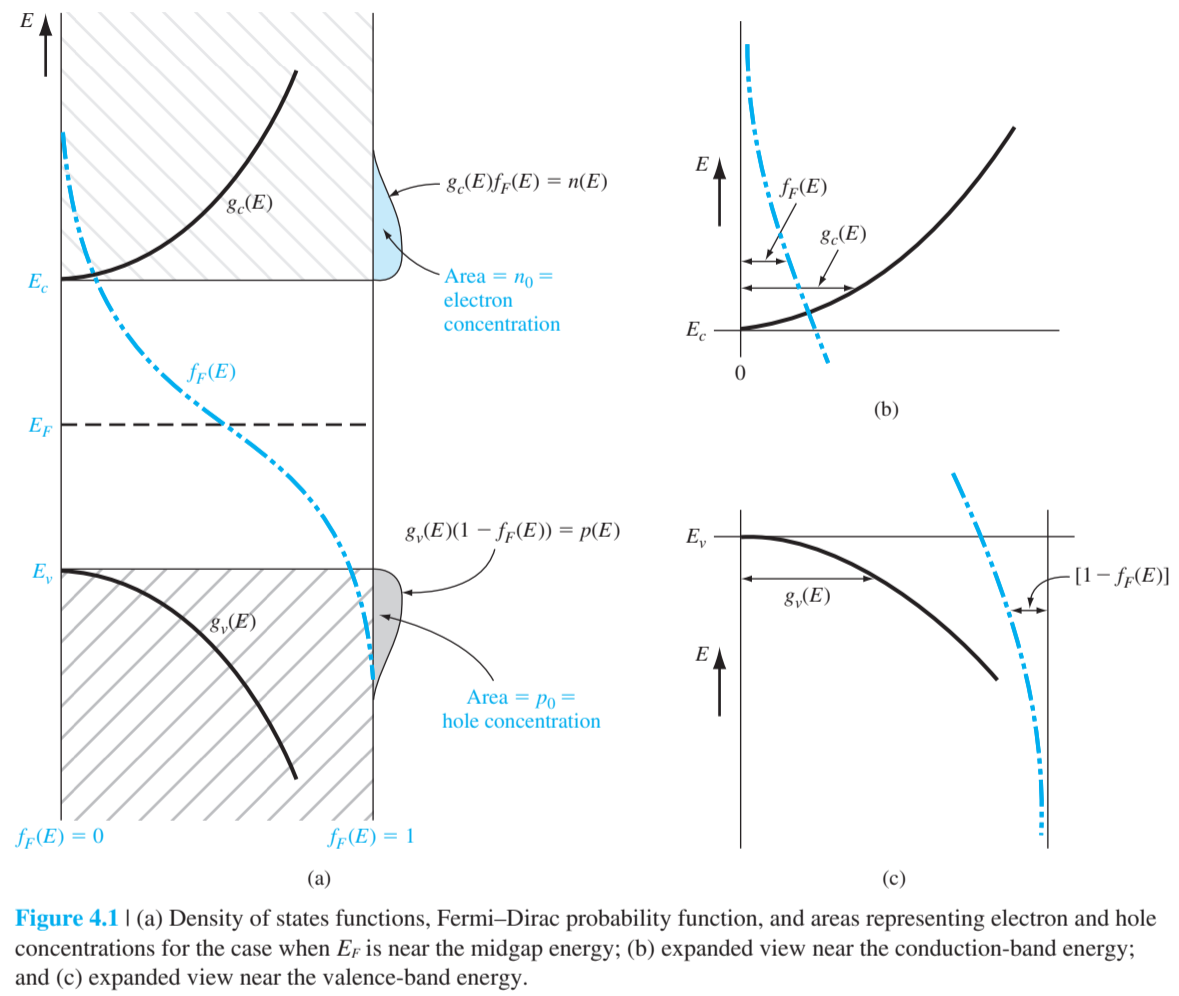
\includegraphics[width=0.7\textwidth]{imagenes/4-1-Semiconductor_intrinseco}
    \caption{Distribución de la densidad de estados $g(E)$, función de Fermi-Dirac $f_F(E)$ y concentraciones de portadores en un semiconductor intrínseco.}
    \label{fig:semiconductor_intrinseco}
\end{figure}

\subsubsection{Semiconductor extrínseco}

Al introducir impurezas dopantes en el semiconductor, la simetría de las concentraciones se rompe manteniendo el producto en equilibrio constante ($n_0 \cdot p_0 = n_i^2$). La incorporación de portadores altera la posición del nivel de Fermi ($E_F$) desplazándolo respecto al nivel intrínseco ($E_{Fi}$):

\begin{itemize}
    \item \textbf{Semiconductor tipo N ($n_0 \gg p_0$):} El exceso de electrones donados desplaza el nivel de Fermi hacia la Banda de Conducción ($E_F > E_{Fi}$). Gráficamente, al acercarse $E_F$ a $E_C$, la función $f_F(E)$ toma valores mayores en la BC, aumentando el área $n_0$ y reduciendo drásticamente el área $p_0$ en la BV.
    \item \textbf{Semiconductor tipo P ($p_0 \gg n_0$):} La generación de huecos por impurezas aceptadoras desplaza el nivel de Fermi hacia la Banda de Valencia ($E_F < E_{Fi}$). Al acercarse $E_F$ a $E_V$, la probabilidad $1 - f_F(E)$ aumenta en la BV, incrementando el área $p_0$ y haciendo insignificante el área $n_0$.
\end{itemize}

\begin{figure}[h!]
    \centering
    \begin{minipage}{0.48\textwidth}
        \centering
        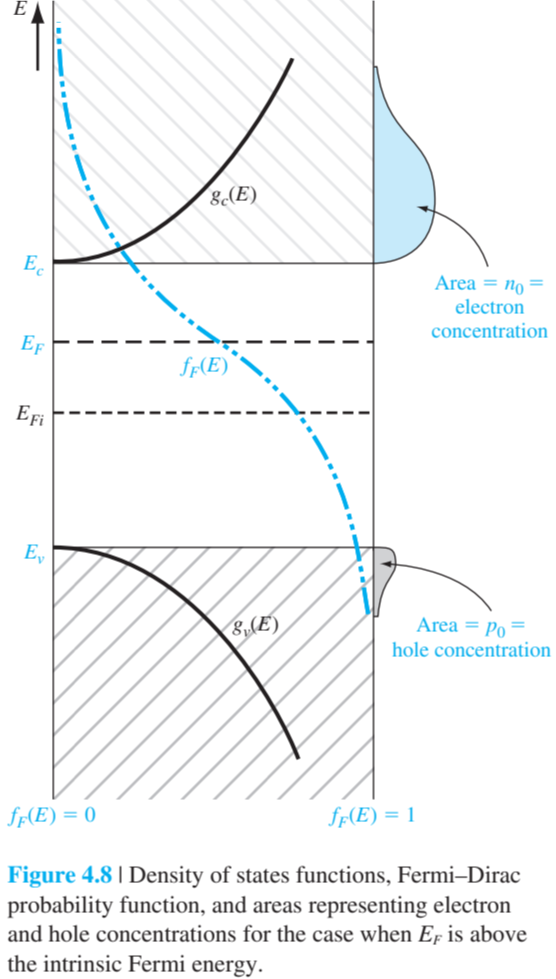
\includegraphics[width=\textwidth]{imagenes/4-8-Semiconductor_extrinseco_a}
        \caption{Semiconductor extrínseco tipo N ($E_F > E_{Fi}$).}
        \label{fig:extrinseco_tipo_n}
    \end{minipage}\hfill
    \begin{minipage}{0.48\textwidth}
        \centering
        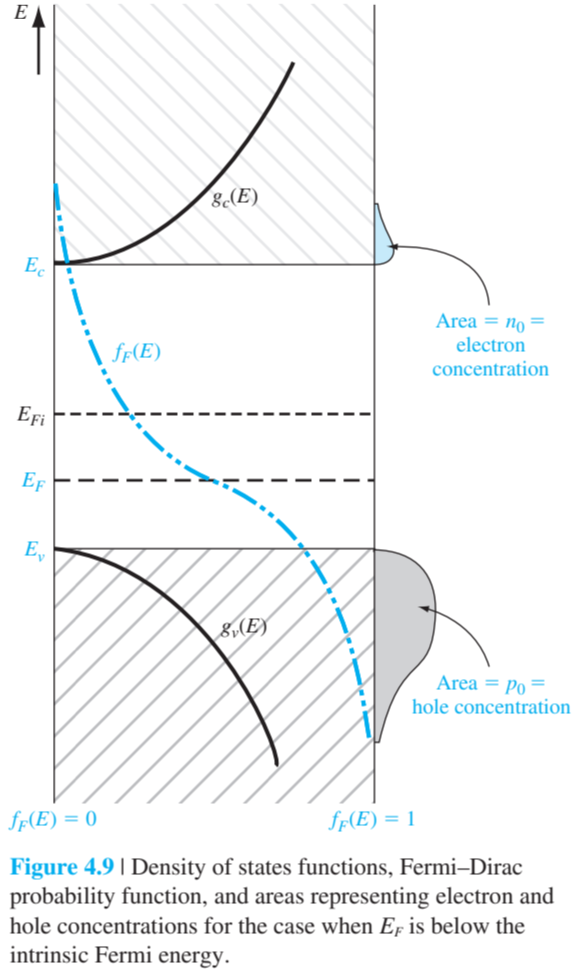
\includegraphics[width=\textwidth]{imagenes/4-9-Semiconductor_extrinseco_b}
        \caption{Semiconductor extrínseco tipo P ($E_F < E_{Fi}$).}
        \label{fig:extrinseco_tipo_p}
    \end{minipage}
\end{figure}

\subsubsection{Semiconductores no degenerados}

Un semiconductor se clasifica como \textbf{no degenerado} cuando la concentración de impurezas dopantes es moderada. En este régimen:
\begin{itemize}
    \item El nivel de Fermi $E_F$ se sitúa dentro de la banda prohibida a una distancia superior a $3 k_B T$ de los bordes de ambas bandas ($E_C - E_F > 3 k_B T$ y $E_F - E_V > 3 k_B T$).
    \item Los estados de la Banda de Conducción están muy poco ocupados por electrones y los de la Banda de Valencia muy poco vacíos de huecos.
    \item Es totalmente válida la aproximación de la estadística de Fermi-Dirac por la de Maxwell-Boltzmann.
\end{itemize}

\begin{figure}[h!]
    \centering
    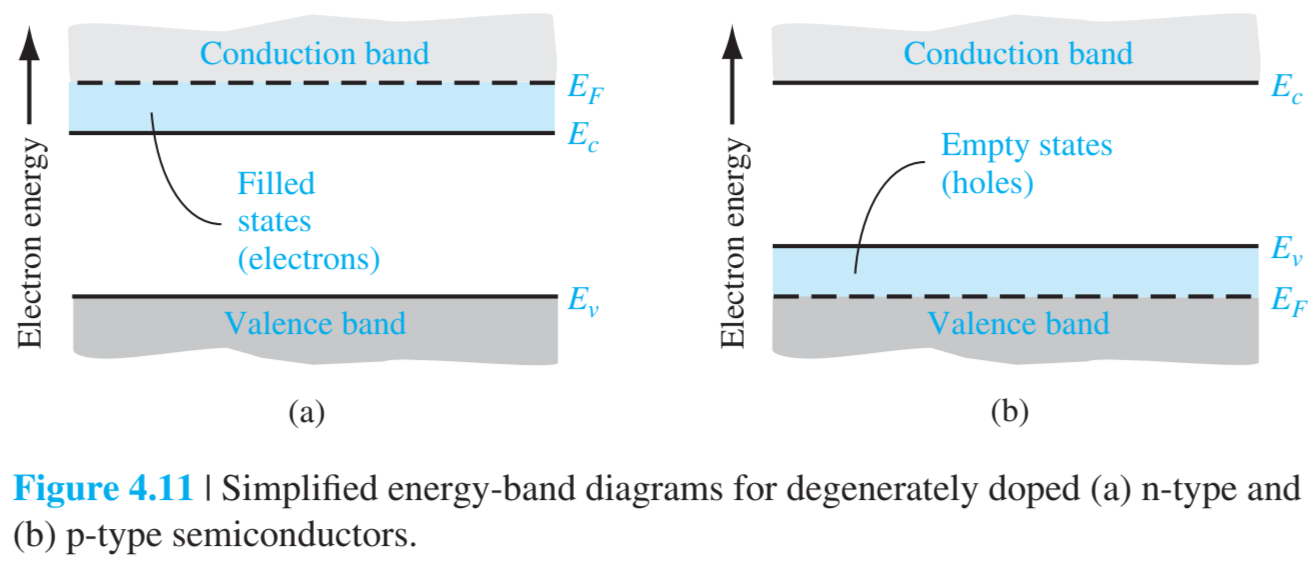
\includegraphics[width=0.65\textwidth]{imagenes/4-11-Semiconductor_degenerado}
    \caption{Diagrama de bandas simplificado para semiconductores no degenerados con el nivel de Fermi dentro del gap.}
    \label{fig:semiconductor_no_degenerado}
\end{figure}

\newpage

$\phantom{a}$

\newpage

\subsubsection{Semiconductores degenerados}

Cuando la concentración de dopante es extremadamente elevada ($N_D > N_c$ o $N_A > N_v$), el material pasa al régimen de \textbf{semiconductor degenerado}:
\begin{itemize}
    \item En materiales tipo N fuertemente dopados ($n^+$), el nivel de Fermi ingresa dentro de la propia Banda de Conducción ($E_F > E_C$).
    \item En materiales tipo P fuertemente dopados ($p^+$), el nivel de Fermi ingresa dentro de la propia Banda de Valencia ($E_F < E_V$).
    \item Todos los estados cuánticos situados por debajo de $E_F$ quedan densamente ocupados por electrones. Ya no resulta aplicable la aproximación de Maxwell-Boltzmann y es obligatorio utilizar la función de Fermi-Dirac completa.
    \item El comportamiento eléctrico del semiconductor degenerado se aproxima al de un conductor metálico.
\end{itemize}

\begin{figure}[h!]
    \centering
    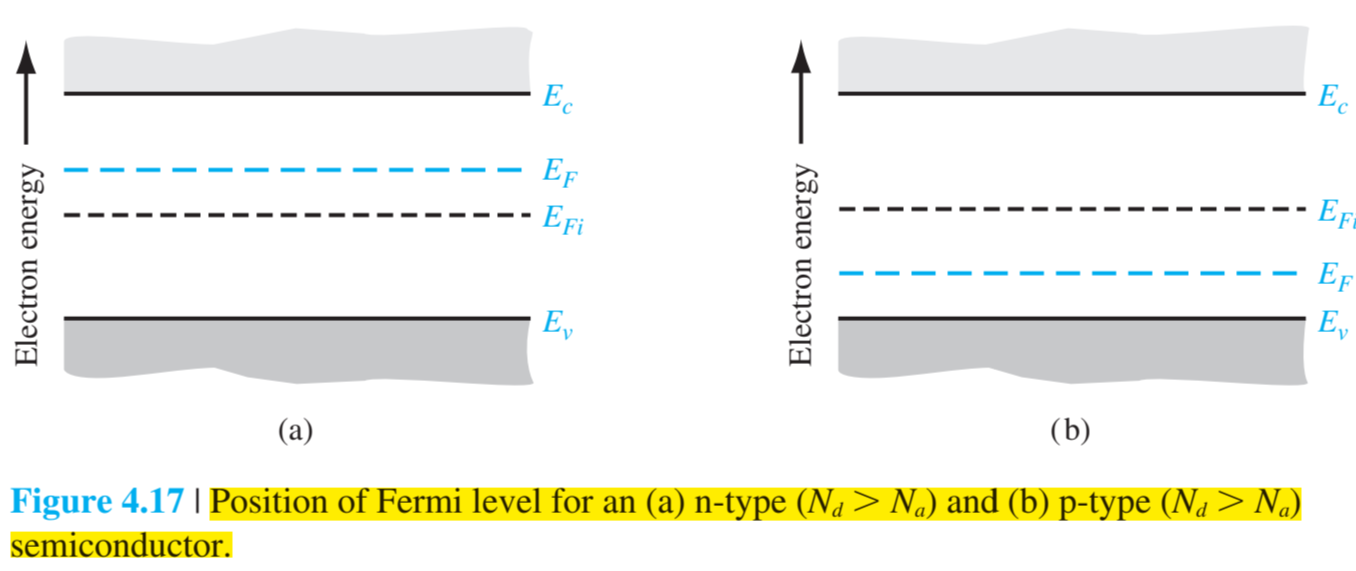
\includegraphics[width=0.9\textwidth]{imagenes/4-17-Semiconductor_nivel_Fermi}
    \caption{Posición del nivel de Fermi dentro de las bandas permitidas en semiconductores degenerados.}
    \label{fig:semiconductor_degenerado}
\end{figure}

\newpage

\begin{problema}[Cálculo de concentraciones de electrones y huecos a partir del nivel de Fermi]
Determinar las concentraciones de electrones ($n_0$) y huecos ($p_0$) en equilibrio térmico para una muestra de Silicio a $T = \SI{300}{\kelvin}$.

\textbf{Datos:}
\begin{itemize}
    \item Densidades equivalentes de estados a \SI{300}{\kelvin}: $N_c = \SI{2.8e19}{\cm^{-3}}$ y $N_v = \SI{1.04e19}{\cm^{-3}}$.
    \item El nivel de Fermi se sitúa a \SI{0.25}{\eV} por debajo del fondo de la banda de conducción ($E_C - E_F = \SI{0.25}{\eV}$).
    \item La anchura de la banda prohibida del Silicio es $E_g = E_C - E_V = \SI{1.12}{\eV}$, por lo que el nivel de Fermi se encuentra a \SI{0.87}{\eV} por encima de la banda de valencia ($E_F - E_V = \SI{0.87}{\eV}$).
    \item Energía térmica a \SI{300}{\kelvin}: $k_B T = \SI{0.0259}{\eV}$.
\end{itemize}

\tcblower

\textbf{1. Concentración de electrones en la banda de conducción ($n_0$)}

Utilizando la aproximación de Maxwell-Boltzmann para semiconductores no degenerados:
\[
n_0 = N_c \exp\left( -\frac{E_C - E_F}{k_B T} \right)
\]

Sustituyendo los datos numéricos:
\[
n_0 = (\SI{2.8e19}{\cm^{-3}}) \exp\left( -\frac{0.25}{0.0259} \right) = \SI{1.8e15}{\cm^{-3}}
\]

\textbf{2. Concentración de huecos en la banda de valencia ($p_0$)}

De forma análoga, la densidad de huecos en equilibrio es:
\[
p_0 = N_v \exp\left( -\frac{E_F - E_V}{k_B T} \right)
\]

Sustituyendo los valores numéricos:
\[
p_0 = (\SI{1.04e19}{\cm^{-3}}) \exp\left( -\frac{0.87}{0.0259} \right) = \SI{2.7e4}{\cm^{-3}}
\]

\textbf{3. Comentario físico}

El desplazamiento del nivel de Fermi unas pocas décimas de electronvoltio respecto a la posición intrínseca modifica la concentración de portadores mayoritarios y minoritarios en varios órdenes de magnitud con respecto a la densidad intrínseca ($n_i \approx \SI{1.5e10}{\cm^{-3}}$).
\end{problema}

\newpage

\subsection{Densidad de portadores y nivel de Fermi en función de la temperatura}

\subsubsection{1. Semiconductor intrínseco}

En un semiconductor intrínseco, las concentraciones de electrones y huecos son iguales a la densidad intrínseca:
\[
n = p = n_i = (N_c N_v)^{1/2} \exp\left( \frac{E_V - E_C}{2 k_B T} \right)
\]

Expresando la densidad de electrones en función de la posición del nivel de Fermi intrínseco ($E_{Fi}$):
\[
n = N_c \exp\left( \frac{E_F - E_C}{k_B T} \right) \iff E_F - E_C = k_B T \ln\left( \frac{n}{N_c} \right)
\]

Igualando $n = n_i$ y despejando la posición del nivel de Fermi intrínseco $E_{Fi}$ respecto al centro de la banda prohibida:
\[
E_{Fi} = \frac{E_C + E_V}{2} + \frac{k_B T}{2} \ln\left( \frac{N_v}{N_c} \right)
\]

\begin{concepto}[Condición de simetría en el centro del gap]
El nivel de Fermi intrínseco $E_{Fi}$ se sitúa exactamente en el centro geométrico del gap ($E_{Fi} = \frac{E_C + E_V}{2}$) únicamente cuando las densidades equivalentes de estados son idénticas ($N_c = N_v$), lo que equivale a que las masas efectivas de electrones y huecos coincidan ($m_n^* = m_p^*$).
\end{concepto}

\subsubsection{2. Semiconductor extrínseco}

En un semiconductor extrínseco dopado con densidades de impurezas donadoras ($N_D$) y aceptadoras ($N_A$), las concentraciones de portadores en equilibrio no degenerado vienen dadas por:
\[
n = N_c \exp\left( \frac{E_F - E_C}{k_B T} \right), \quad p = N_v \exp\left( \frac{E_V - E_F}{k_B T} \right)
\]
cumpliéndose en todo momento la \textbf{ley de acción de masas}:
\[
n \cdot p = n_i^2
\]

La ocupación parcial de los niveles de impurezas viene determinada por:
\[
\frac{N_D^+}{N_D^0} = \frac{1}{g_d} \exp\left( \frac{E_D - E_F}{k_B T} \right), \quad \frac{N_A^-}{N_A^0} = \frac{1}{g_a} \exp\left( \frac{E_F - E_A}{k_B T} \right)
\]

La posición del nivel de Fermi $E_F$ queda unívocamente determinada por la \textbf{condición de neutralidad de carga eléctrica} macroscópica del cristal:
\[
p + N_D^+ = n + N_A^-
\]

\paragraph{Caso 1: Ionización total de impurezas}

A temperatura ambiente ($T = \SI{300}{\kelvin}$), la energía térmica es suficiente para ionizar la práctica totalidad de las impurezas sustitucionales presentes ($N_D^+ = N_D$ y $N_A^- = N_A$). La condición de neutralidad y la ley de acción de masas forman un sistema de dos ecuaciones algebraicas con dos incógnitas ($n$ y $p$):
\[
\left\{
\begin{array}{l}
n \cdot p = n_i^2 \\
p + N_D = n + N_A
\end{array}
\right\}
\]

Sustituyendo $p = \frac{n_i^2}{n}$ en la ecuación de neutralidad se obtiene la ecuación cuadrática:
\[
n^2 - (N_D - N_A) n - n_i^2 = 0
\]

Tomando la solución físicamente válida (concentración de electrones positiva):
\[
n = \frac{N_D - N_A}{2} + \sqrt{\left(\frac{N_D - N_A}{2}\right)^2 + n_i^2}
\]

\begin{concepto}[Aproximación de portadores minoritarios despreciables]
En la mayoría de los casos prácticos con dopado moderado o elevado, la densidad neta de impurezas es mucho mayor que la concentración intrínseca ($N_D - N_A \gg n_i$). En esta situación no es necesario resolver la ecuación cuadrática completa:
\begin{itemize}
    \item La densidad de portadores mayoritarios se aproxima directamente por la densidad de dopado neto:
    \[
    n \approx N_D - N_A
    \]
    \item La densidad de portadores minoritarios resulta extremadamente pequeña frente a las impurezas:
    \[
    p = \frac{n_i^2}{n} \approx \frac{n_i^2}{N_D - N_A} \ll N_D - N_A
    \]
\end{itemize}
\end{concepto}

\newpage

\begin{problema}[Concentraciones de portadores en Silicio dopado]
Determinar las concentraciones de electrones ($n_0$) y huecos ($p_0$) en equilibrio térmico para muestras de Silicio a $T = \SI{300}{\kelvin}$ sometidas a las siguientes concentraciones de dopado:
\begin{enumerate}
    \item $N_D = \SI{1e16}{\cm^{-3}}$ y $N_A = 0$.
    \item $N_D = \SI{5e15}{\cm^{-3}}$ y $N_A = \SI{2e15}{\cm^{-3}}$.
\end{enumerate}

\textbf{Datos:}
\begin{itemize}
    \item Densidad intrínseca del Silicio a $T = \SI{300}{\kelvin}$: $n_i = \SI{1.5e10}{\cm^{-3}}$.
\end{itemize}

\tcblower

\textbf{1. Apartado a)}

Aplicando la expresión general para la concentración de electrones mayoritarios con $N_D - N_A = \SI{1e16}{\cm^{-3}}$ :
\[
n_0 = \frac{10^{16}}{2} + \sqrt{\left(\frac{10^{16}}{2}\right)^2 + (\num{1.5e10})^2} \approx \SI{1e16}{\cm^{-3}}
\]

La densidad de huecos minoritarios se obtiene mediante la ley de acción de masas:
\[
p_0 = \frac{n_i^2}{n_0} = \frac{(\num{1.5e10})^2}{10^{16}} = \SI{2.25e4}{\cm^{-3}}
\]

\textbf{2. Apartado b)}

Con un dopado neto de $N_D - N_A = \SI{5e15}{\cm^{-3}} - \SI{2e15}{\cm^{-3}} = \SI{3e15}{\cm^{-3}}$:
\[
n_0 = \frac{\num{3e15}}{2} + \sqrt{\left(\frac{\num{3e15}}{2}\right)^2 + (\num{1.5e10})^2} \approx \SI{3e15}{\cm^{-3}}
\]

La concentración de huecos minoritarios resulta:
\[
p_0 = \frac{n_i^2}{n_0} = \frac{(\num{1.5e10})^2}{\num{3e15}} = \SI{7.5e4}{\cm^{-3}}
\]

\textbf{3. Comentario físico}

En ambos casos se cumple $N_D - N_A \gg n_i$, por lo que la concentración de portadores mayoritarios en equilibrio es prácticamente igual a la diferencia entre las concentraciones de donadores y aceptadores ($n_0 \approx N_D - N_A$). Asimismo, la densidad de mayoritarios es varios órdenes de magnitud superior a la de minoritarios.
\end{problema}

\newpage

\begin{problema}[Concentración de portadores en Germanio con dopado moderado]
Calcular las concentraciones de electrones ($n_0$) y huecos ($p_0$) en equilibrio térmico a $T = \SI{300}{\kelvin}$ para una muestra de Germanio dopada con $N_D = \SI{2e14}{\cm^{-3}}$ y $N_A = 0$.

\textbf{Datos:}
\begin{itemize}
    \item Densidad intrínseca del Germanio a $T = \SI{300}{\kelvin}$: $n_i = \SI{2.4e13}{\cm^{-3}}$.
\end{itemize}

\tcblower

A diferencia del Silicio, la densidad intrínseca del Germanio es significativamente mayor, por lo que el término $n_i$ no es despreciable frente al dopado $N_D = \SI{2e14}{\cm^{-3}}$.

Calculamos la densidad de electrones mediante la expresión exacta:
\[
n_0 = \frac{\num{2e14}}{2} + \sqrt{\left(\frac{\num{2e14}}{2}\right)^2 + (\num{2.4e13})^2} \approx \SI{2.028e14}{\cm^{-3}}
\]

La densidad de huecos minoritarios resulta:
\[
p_0 = \frac{n_i^2}{n_0} = \frac{(\num{2.4e13})^2}{\num{2.028e14}} \approx \SI{2.84e12}{\cm^{-3}}
\]

\textbf{Comentario físico}

Cuando la concentración de impurezas donadoras no es mucho mayor que la densidad intrínseca (misma escala de magnitud), la generación térmica aporta una fracción apreciable a la concentración total de mayoritarios, haciendo necesario el cálculo exacto sin aproximaciones.
\end{problema}

\subsection{Densidad de portadores y nivel de Fermi en función de la temperatura}

\subsubsection{1. Semiconductor intrínseco}

En un semiconductor intrínseco, la densidad de portadores generados térmicamente sigue la relación:
\[
n = p = n_i = \sqrt{N_c N_v} \exp\left( -\frac{E_g}{2 k_B T} \right)
\]
A medida que la temperatura aumenta, la generación térmica domina y la concentración de portadores crece exponencialmente.

\subsubsection{2. Semiconductor extrínseco}

\paragraph{Caso 1: Ionización total de impurezas}

A temperaturas moderadas (como la temperatura ambiente, $T = \SI{300}{\kelvin}$), todas las impurezas introducidas se encuentran totalmente ionizadas ($N_D^+ = N_D$ y $N_A^- = N_A$). El problema de determinar la densidad de portadores se reduce a un sistema de dos ecuaciones con dos incógnitas:
\[
\left\{
\begin{array}{l}
n \cdot p = n_i^2 \\
p + N_D = n + N_A
\end{array}
\right\} 
\implies n = \frac{N_D - N_A}{2} + \sqrt{\left(\frac{N_D - N_A}{2}\right)^2 + n_i^2}
\]

\begin{concepto}[Aproximación para portadores minoritarios despreciables]
En la mayoría de aplicaciones prácticas donde la densidad de dopado supera ampliamente a la concentración intrínseca ($N_D - N_A \gg n_i$), no es necesario resolver el sistema cuadrático completo:
\begin{itemize}
    \item La densidad de portadores mayoritarios queda determinada directamente por la densidad de impurezas ionizadas:
    \[
    n \approx N_D - N_A
    \]
    \item La densidad de portadores minoritarios resulta insignificante frente al dopado:
    \[
    p = \frac{n_i^2}{n} \approx \frac{n_i^2}{N_D - N_A} \ll N_D - N_A
    \]
\end{itemize}
\end{concepto}

\newpage

\subsection{Concentración de portadores en función de la temperatura}

La concentración de portadores libres en un semiconductor extrínseco varía sustancialmente con la temperatura. Analizando el caso de un semiconductor tipo N dopado con una densidad de donadores $N_D$, la curva de concentración de electrones $n_0(T)$ exhibe tres regiones claramente diferenciadas:

\begin{enumerate}
    \item \textbf{Región de ionización parcial o congelación de portadores (\textit{Freeze-out}):} 
    A temperaturas muy bajas ($T \to \SI{0}{\kelvin}$), la energía térmica $k_B T$ es insuficiente para superar la energía de ionización $\Delta E = E_C - E_D$. Los electrones permanecen ligados a los átomos de impureza en el nivel donador $E_D$. A medida que la temperatura asciende, los donadores comienzan a ionizarse de forma progresiva:
    \[
    n_0 \approx N_D^+ < N_D, \quad p_0 = \frac{n_i^2}{N_D^+}
    \]

    \item \textbf{Región extrínseca o de agotamiento (\textit{Exhaustion region}):} 
    Es el intervalo térmico de operación de interés para los dispositivos electrónicos (típicamente entre \SI{100}{\kelvin} y \SI{450}{\kelvin} en Silicio). En este rango, la energía térmica es suficiente para ionizar el $100\%$ de las impurezas ($N_D^+ = N_D$), pero aún no es bastante alta para generar una cantidad significativa de pares electrón-hueco intrínsecos. La densidad de mayoritarios se mantiene prácticamente constante e igual al dopado:
    \[
    n_0 \approx N_D, \quad p_0 = \frac{n_i^2}{N_D}
    \]

    \item \textbf{Región intrínseca:} 
    A temperaturas elevadas ($T > \SI{500}{\kelvin}$ en Silicio con dopado moderado), la concentración intrínseca de portadores $n_i(T) \propto T^{3/2} \exp\left(-\frac{E_g}{2 k_B T}\right)$ crece exponencialmente hasta superar ampliamente la densidad de dopado ($n_i \gg N_D$). La generación térmica banda a banda domina por completo el comportamiento del material:
    \[
    n_0 \approx p_0 \approx n_i = \sqrt{N_c N_v} \exp\left( -\frac{E_g}{2 k_B T} \right)
    \]
\end{enumerate}

\begin{figure}[h!]
    \centering
    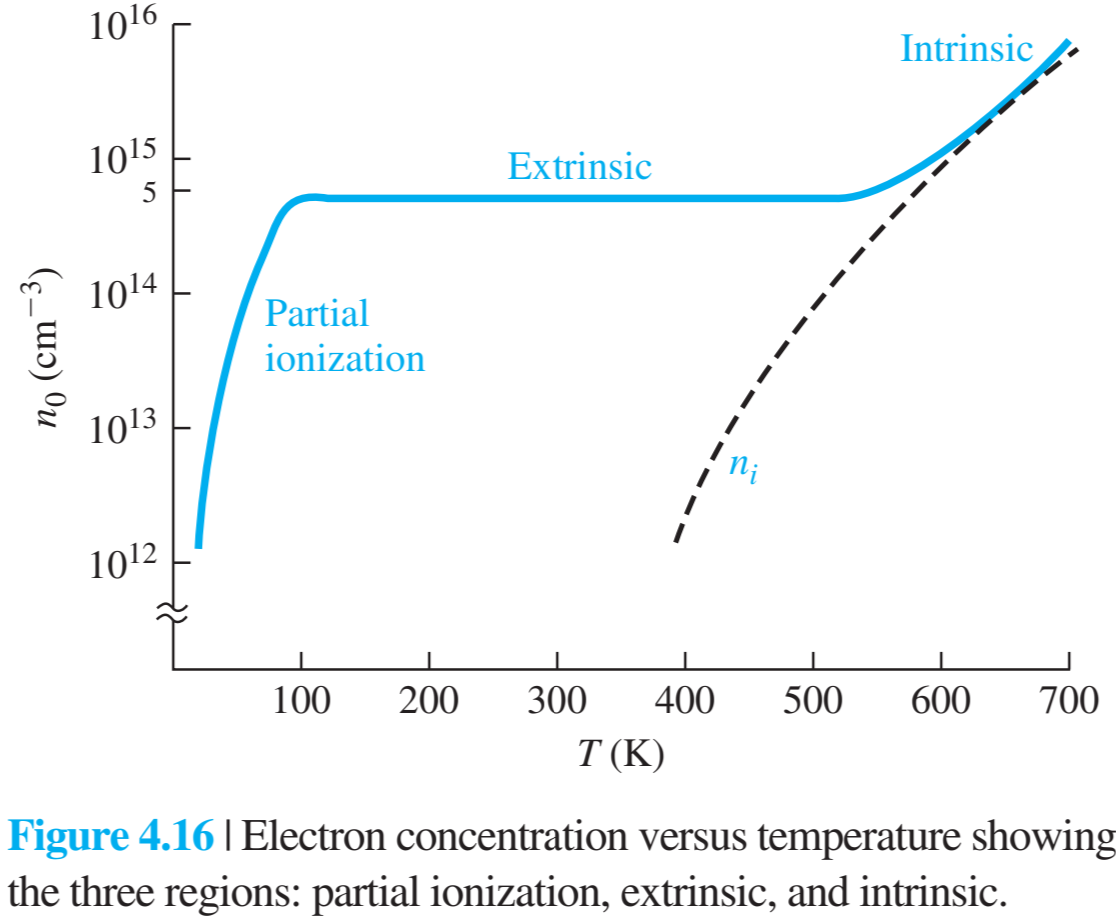
\includegraphics[width=0.4\textwidth]{imagenes/4-16-Concentracion_vs_temperatura}
    \caption{Concentración de electrones en función de la temperatura para un semiconductor tipo N, mostrando las regiones de ionización parcial, extrínseca e intrínseca.}
    \label{fig:concentracion_vs_temperatura}
\end{figure}

\newpage

\subsection{Nivel de Fermi en función de la temperatura}

La posición energética del nivel de Fermi ($E_F$) evoluciona con la temperatura debido a dos factores contrapuestos: la variación de la ionización de las impurezas y la dependencia de las densidades equivalentes de estados ($N_c, N_v \propto T^{3/2}$).

A partir de las expresiones para la densidad de portadores no degenerados:
\[
E_C - E_F = k_B T \ln\left( \frac{N_c}{n_0} \right), \quad E_F - E_V = k_B T \ln\left( \frac{N_v}{p_0} \right)
\]

\begin{concepto}[Evolución del nivel de Fermi con $T$]
\begin{itemize}
    \item \textbf{Cero absoluto ($T = \SI{0}{\kelvin}$):} En un semiconductor tipo N, el nivel de Fermi se sitúa exactamente a la mitad de la separación entre el nivel donador y la Banda de Conducción ($E_F = \frac{E_C + E_D}{2}$). En un semiconductor tipo P, se ubica en el punto medio entre la Banda de Valencia y el nivel aceptador ($E_F = \frac{E_V + E_A}{2}$).
    \item \textbf{Región extrínseca ($T \approx \SI{300}{\kelvin}$):} Al ionizarse las impurezas, $E_F$ se sitúa próximo a $E_C$ en materiales tipo N, o próximo a $E_V$ en materiales tipo P. Al aumentar la temperatura dentro de esta región, el término $k_B T \ln(N_c / N_D)$ desplaza progresivamente a $E_F$ hacia el centro del gap.
    \item \textbf{Región intrínseca ($T$ elevada):} Cuando la generación térmica domina ($n_i \gg N_D, N_A$), el nivel de Fermi de cualquier semiconductor (sea tipo N o tipo P) converge asintóticamente hacia la posición del nivel de Fermi intrínseco ($E_F \to E_{Fi}$).
\end{itemize}
\end{concepto}

\begin{figure}[h!]
    \centering
    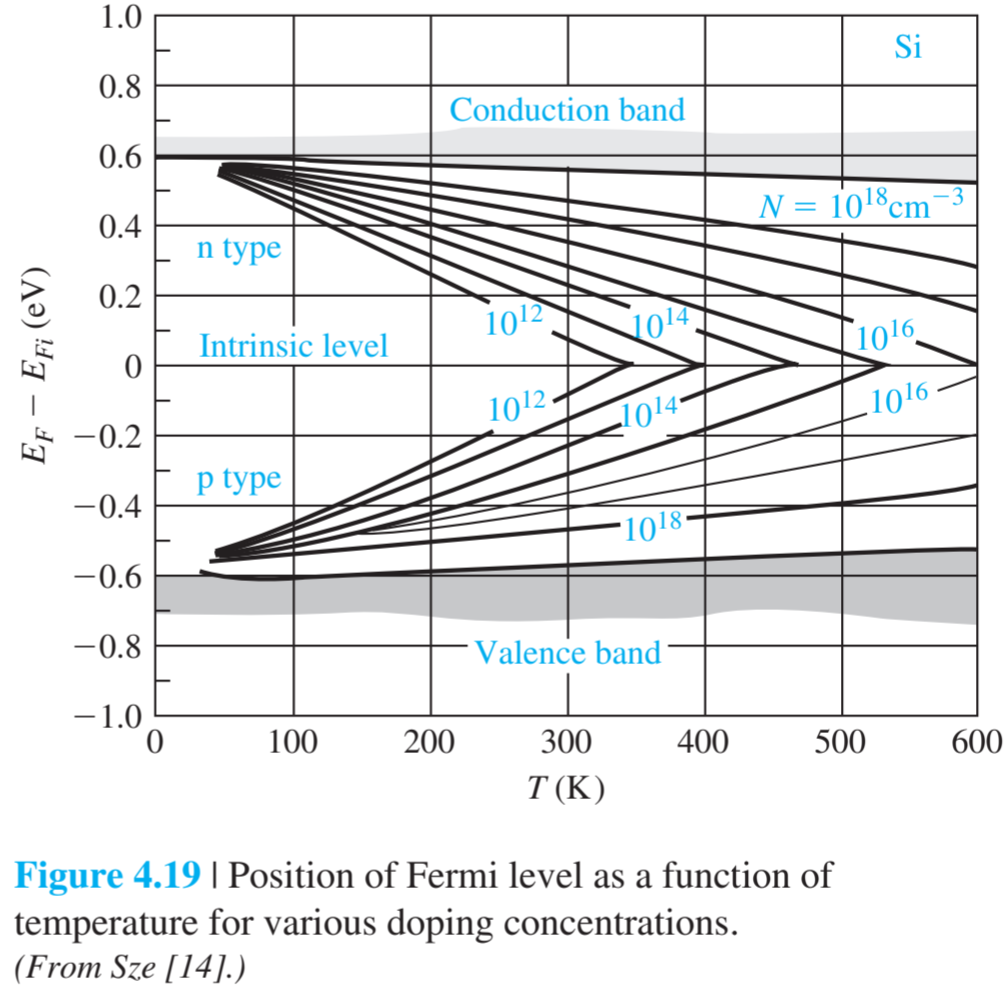
\includegraphics[width=0.6\textwidth]{imagenes/4-19-Nivel_Fermi_vs_Temperatura}
    \caption{Posición del nivel de Fermi ($E_F - E_{Fi}$) en función de la temperatura en Silicio para diversas concentraciones de dopado tipo N y tipo P.}
    \label{fig:nivel_fermi_vs_temperatura}
\end{figure}

\newpage

\subsection{Nivel de Fermi en función de la concentración de impurezas}

En la región extrínseca o de agotamiento (a temperatura ambiente constante $T = \SI{300}{\kelvin}$), la posición del nivel de Fermi queda fijada exclusivamente por la densidad de dopado introducida en el cristal.

Relacionando la densidad de portadores mayoritarios con el nivel de Fermi intrínseco ($E_{Fi}$):
\[
n_0 = n_i \exp\left( \frac{E_F - E_{Fi}}{k_B T} \right) \implies E_F - E_{Fi} = k_B T \ln\left( \frac{n_0}{n_i} \right)
\]
\[
p_0 = n_i \exp\left( \frac{E_{Fi} - E_F}{k_B T} \right) \implies E_{Fi} - E_F = k_B T \ln\left( \frac{p_0}{n_i} \right)
\]

Bajo ionización total ($n_0 \approx N_D$ y $p_0 \approx N_A$):

\begin{formula}[Desplazamiento de $E_F$ con la densidad de dopado]
\begin{itemize}
    \item \textbf{Semiconductor tipo N:}
    \[
    E_F - E_{Fi} = k_B T \ln\left( \frac{N_D}{n_i} \right) \quad \text{o bien} \quad E_C - E_F = k_B T \ln\left( \frac{N_c}{N_D} \right)
    \]
    A mayor concentración de donadores $N_D$, el nivel de Fermi se aproxima más al fondo de la Banda de Conducción $E_C$.
    \item \textbf{Semiconductor tipo P:}
    \[
    E_{Fi} - E_F = k_B T \ln\left( \frac{N_A}{n_i} \right) \quad \text{o bien} \quad E_F - E_V = k_B T \ln\left( \frac{N_v}{N_A} \right)
    \]
    A mayor concentración de aceptadores $N_A$, el nivel de Fermi se aproxima más al techo de la Banda de Valencia $E_V$.
\end{itemize}
\end{formula}

\begin{figure}[h!]
    \centering
    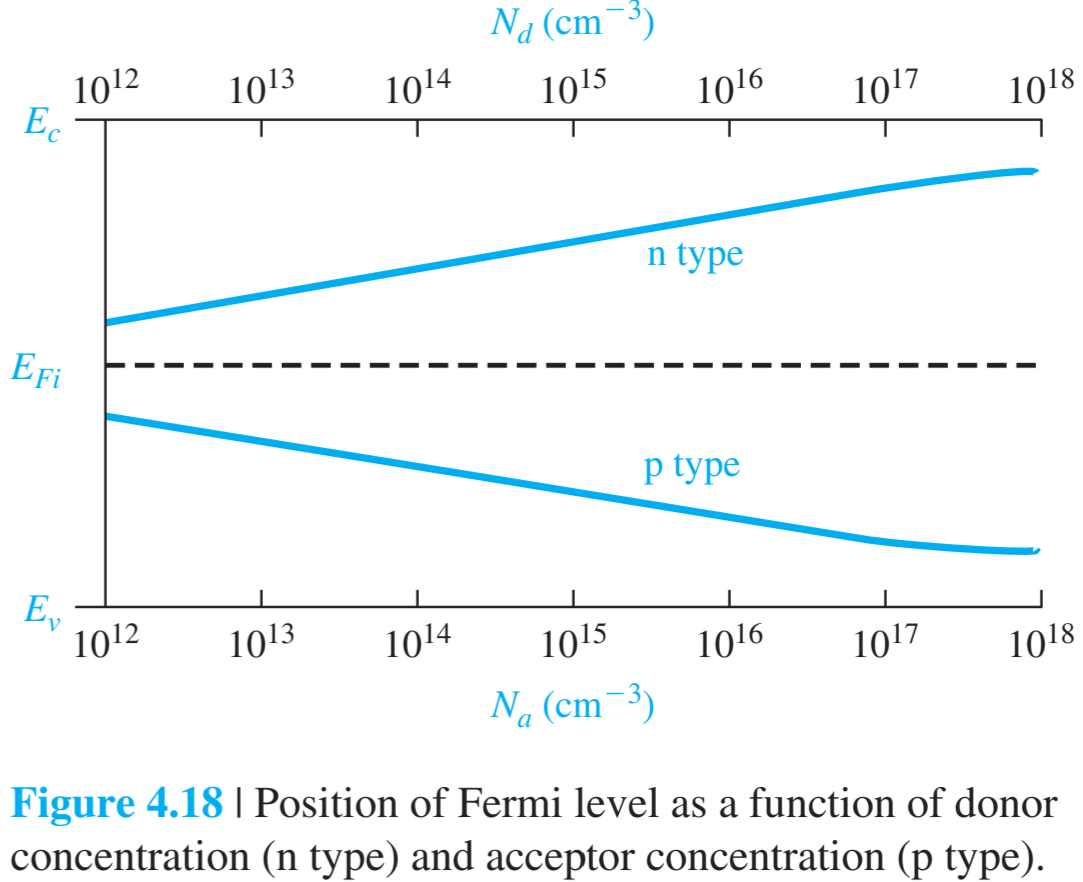
\includegraphics[width=0.6\textwidth]{imagenes/4-18-Nivel_Fermi_vs_Concentracion}
    \caption{Posición del nivel de Fermi respecto al nivel intrínseco en función de la densidad de impurezas donadoras ($N_D$) y aceptadoras ($N_A$). Se indica la transición al régimen degenerado para concentraciones muy elevadas.}
    \label{fig:nivel_fermi_vs_concentracion}
\end{figure}

\begin{concepto}[Límite de degeneración por dopado]
Si la concentración de donadores se incrementa hasta alcanzar o superar la densidad equivalente de estados ($N_D \ge N_c$), el nivel de Fermi alcanza el borde de la banda ($E_F \ge E_C$) y penetra en la Banda de Conducción. El semiconductor entra en el régimen \textbf{degenerado}, adquiriendo propiedades conductoras similares a las de un metal. De forma simétrica, si $N_A \ge N_v$, $E_F$ penetra en la Banda de Valencia ($E_F \le E_V$).
\end{concepto}

\newpage
\phantom{a}

\newpage
%=======================================================
\seccionproblemas
%-----------------------------------------------------
%-------------- Problema 1 ---------------------------
%-----------------------------------------------------
\begin{problema}[Densidades de portadores en Silicio dopado tipo N]
Una muestra de Silicio ($\text{Si}$) está impurificada con $10^{15} \text{ átomos/cm}^3$ de Fósforo ($\text{P}$, impureza donadora). Suponiendo que todos estos átomos de impureza están ionizados a temperatura ambiente, hallar las densidades de portadores (electrones y huecos) en dicho material.

\textbf{Datos:}
\begin{itemize}
    \item Densidad de donadores: $N_D = \SI{1e15}{\cm^{-3}}$.
    \item Densidad intrínseca del Silicio a temperatura ambiente: $n_i = \SI{1.45e10}{\cm^{-3}}$.
\end{itemize}

\tcblower

\textbf{1. Planteamiento de ecuaciones fundamentales}

En un semiconductor en equilibrio térmico rigen dos ecuaciones básicas:
\begin{enumerate}
    \item \textbf{Ley de acción de masas:}
    \[
    n \cdot p = n_i^2
    \]
    \item \textbf{Condición de neutralidad de carga eléctrica:}
    Dado que no hay impurezas aceptadoras ($N_A = 0$) y considerando ionización total de donadores ($N_D^+ = N_D$):
    \[
    n = p + N_D
    \]
\end{enumerate}

\textbf{2. Justificación de la aproximación de portadores minoritarios}

Despejando la concentración de huecos ($p$) de la ley de acción de masas:
\[
p = \frac{n_i^2}{n}
\]

Dado que la presencia de donadores incrementa la concentración de electrones ($n > N_D$), podemos acotar superiormente la densidad de huecos:
\[
p = \frac{n_i^2}{n} < \frac{n_i^2}{N_D} = \frac{(\num{1.45e10})^2}{10^{15}} = \SI{2.1025e5}{\cm^{-3}} \approx \SI{2.10e5}{\cm^{-3}}
\]

Comparando este valor límite con la concentración de dopado:
\[
p \approx \SI{2.10e5}{\cm^{-3}} \ll N_D = \SI{1e15}{\cm^{-3}}
\]

Puesto que $p$ es completamente despreciable frente a $N_D$, la condición de neutralidad $n = p + N_D$ se simplifica a:
\[
n \approx N_D = \SI{1e15}{\cm^{-3}}
\]

\textbf{3. Cálculo de la densidad de huecos ($p$)}

Sustituyendo $n = \SI{1e15}{\cm^{-3}}$ en la ley de acción de masas:
\[
p = \frac{n_i^2}{n} = \frac{(\num{1.45e10})^2}{10^{15}} = \SI{2.10e5}{\cm^{-3}}
\]

\textbf{4. Verificación mediante la solución exacta}

Sustituyendo $p = \frac{n_i^2}{n}$ en la condición de neutralidad $n = p + N_D$ obtenemos la ecuación cuadrática:
\[
n^2 - N_D n - n_i^2 = 0
\]

Tomando la solución física positiva:
\[
n = \frac{N_D}{2} + \sqrt{\left(\frac{N_D}{2}\right)^2 + n_i^2} = \frac{10^{15}}{2} + \sqrt{\left(\frac{10^{15}}{2}\right)^2 + (\num{1.45e10})^2} \approx \SI{1e15}{\cm^{-3}}
\]

Esto confirma que la aproximación $n \approx N_D$ es exacta en la práctica con más de ocho cifras significativas de precisión.

\textbf{Resultado final:}
\begin{itemize}
    \item Concentración de electrones (mayoritarios): $n = \SI{1e15}{\cm^{-3}}$.
    \item Concentración de huecos (minoritarios): $p = \SI{2.10e5}{\cm^{-3}}$.
\end{itemize}
\end{problema}

\newpage
%-----------------------------------------------------
%-------------- Problema 2 ---------------------------
%-----------------------------------------------------
\begin{problema}[Determinar tipo y concentración de dopado]
Un semiconductor presenta concentraciones de portadores $n = \SI{1e18}{\cm^{-3}}$ y $p = \SI{1e6}{\cm^{-3}}$ a $T = \SI{300}{\kelvin}$. ¿Con cuántas impurezas y de qué tipo ha sido dopada la muestra? (Suponer que es dopado por un único tipo de impureza y que todas están completamente ionizadas).

\tcblower

\textbf{1. Determinación del tipo de semiconductor}

Al comparar las concentraciones de portadores en equilibrio:
\[
n = \SI{1e18}{\cm^{-3}} \gg p = \SI{1e6}{\cm^{-3}}
\]
Dado que la densidad de electrones supera ampliamente a la de huecos ($n \gg p$), concluimos que se trata de un \textbf{semiconductor extrínseco tipo N}. Por lo tanto, el dopado se ha realizado mediante \textbf{impurezas donadoras} ($N_D > 0, N_A = 0$).

\textbf{2. Cálculo de la concentración de impurezas donadoras ($N_D$)}

Aplicando la condición de neutralidad eléctrica global para un semiconductor tipo N bajo la hipótesis de ionización total ($N_D^+ = N_D$):
\[
n = p + N_D
\]

Despejando la densidad de donadores $N_D$:
\[
N_D = n - p = \SI{1e18}{\cm^{-3}} - \SI{1e6}{\cm^{-3}}
\]

Puesto que $p = \SI{1e6}{\cm^{-3}}$ es completamente insignificante en comparación con $n = \SI{1e18}{\cm^{-3}}$ (difieren en 12 órdenes de magnitud):
\[
N_D \approx n = \SI{1e18}{\cm^{-3}}
\]

\textbf{Resultado final:}
La muestra ha sido dopada con impurezas de tipo \textbf{donador} (tipo N) en una densidad de $N_D = \SI{1e18}{\cm^{-3}}$.
\end{problema}

\newpage
%-----------------------------------------------------
%-------------- Problema 3 ---------------------------
%-----------------------------------------------------
\begin{problema}[Nivel de Fermi e ionización parcial de donadores]
Una barra de semiconductor tipo N posee las siguientes propiedades a $T = \SI{300}{\kelvin}$ ($k_B T = \SI{0.026}{\eV}$): $N_c = \SI{2e19}{\cm^{-3}}$, $n_i = \SI{2e10}{\cm^{-3}}$, y contiene $N_D = \SI{1e15}{\cm^{-3}}$ átomos de impurezas donadoras por $\text{cm}^3$ con una energía de ionización $E_C - E_D = \SI{0.03}{\eV}$ y factor de degeneración $g_D = 2$.

\begin{enumerate}[label=\alph*)]
    \item Suponiendo que estas impurezas están totalmente ionizadas, determinar la posición del nivel de Fermi respecto al nivel intrínseco ($E_F - E_{Fi}$) a $T = \SI{300}{\kelvin}$.
    \item ¿A qué temperatura estarán ionizados únicamente el $25\%$ de los centros donadores?
\end{enumerate}

\tcblower

Para este tipo de problemas seguimos la metodología estándar: \textbf{Plantear hipótesis} $\to$ \textbf{Resolver bajo dicha suposición} $\to$ \textbf{Comprobar la validez y aceptar/rechazar la hipótesis}.

\textbf{a) Determinación de $E_F - E_{Fi}$ a $T = \SI{300}{\kelvin}$}

\textit{Paso 1: Planteamiento bajo la hipótesis de ionización total.}
Asumimos inicialmente que la totalidad de los donadores están ionizados ($N_D^+ = N_D$). Dado que $N_D \gg n_i$, la concentración de electrones libres es:
\[
n \approx N_D = \SI{1e15}{\cm^{-3}}
\]

\textit{Paso 2: Cálculo de la posición del nivel de Fermi.}
La densidad de electrones en la banda de conducción se expresa como:
\[
n = N_c \exp\left( \frac{E_F - E_C}{k_B T} \right) \implies E_F - E_C = k_B T \ln\left( \frac{N_D}{N_c} \right)
\]
Sustituyendo valores numéricos:
\[
E_F - E_C = (\SI{0.026}{\eV}) \ln\left( \frac{\num{1e15}}{\num{2e19}} \right) = (\SI{0.026}{\eV}) \ln(\num{5e-5}) = \SI{-0.2565}{\eV}
\]

Por otro lado, relacionando la densidad intrínseca $n_i$ con el nivel intrínseco $E_{Fi}$:
\[
n_i = N_c \exp\left( \frac{E_{Fi} - E_C}{k_B T} \right) \implies E_{Fi} - E_C = k_B T \ln\left( \frac{n_i}{N_c} \right)
\]
\[
E_{Fi} - E_C = (\SI{0.026}{\eV}) \ln\left( \frac{\num{2e10}}{\num{2e19}} \right) = (\SI{0.026}{\eV}) \ln(\num{1e-9}) = \SI{-0.3367}{\eV}
\]

Restando ambas ecuaciones obtenemos la posición de $E_F$ respecto a $E_{Fi}$:
\[
E_F - E_{Fi} = (E_F - E_C) - (E_{Fi} - E_C) = \SI{-0.2565}{\eV} - (\SI{-0.3367}{\eV}) = \SI{0.2802}{\eV}
\]

\textit{Nota alternativa directa:} La relación se puede obtener en un solo paso dividiendo las expresiones $n/n_i$:
\[
\frac{n}{n_i} = \exp\left( \frac{E_F - E_{Fi}}{k_B T} \right) \implies 
\]
\[
\implies E_F - E_{Fi} = k_B T \ln\left( \frac{n}{n_i} \right) = (\SI{0.026}{\eV}) \ln\left( \frac{\num{1e15}}{\num{2e10}} \right) = \SI{0.2813}{\eV}
\]

\begin{center}
    
\includegraphics[width=0.6\textwidth]{imagenes/tema2/T2P3.png}
    \captionof{figure}{Diagrama de niveles de energía mostrando la posición relativa de $E_F$ respecto a $E_{Fi}$, $E_C$ y $E_D$.}
    \label{fig:problema_3_diagrama}
\end{center}

\textit{Paso 3: Verificación de la hipótesis de ionización total.}
Calculamos la fracción real de donadores ionizados mediante la estadística de impurezas:
\[
\frac{N_D^+}{N_D} = \frac{1}{1 + g_D \exp\left( \frac{E_F - E_D}{k_B T} \right)}
\]
Donde la separación $E_F - E_D$ es:
\[
E_F - E_D = (E_F - E_C) + (E_C - E_D) = \SI{-0.2565}{\eV} + \SI{0.03}{\eV} = \SI{-0.2265}{\eV}
\]
Sustituyendo en la fracción de ionización:
\[
\frac{N_D^+}{N_D} = \frac{1}{1 + 2 \exp\left( \frac{-0.2265}{0.026} \right)} = \frac{1}{1 + 2 \exp(-8.7115)} = \frac{1}{1 + \num{0.000329}} \approx 0.9997
\]
Puesto que el $99.97\%$ ($\approx 0.9991$) de las impurezas están ionizadas, la hipótesis planteada es \textbf{completamente válida} y la solución queda aceptada.

\textbf{b) Temperatura para un $25\%$ de ionización donadora}

Buscamos la temperatura $T$ tal que la fracción ionizada sea $\frac{N_D^+}{N_D} = 0.25$, lo que implica que los donadores neutros (no ionizados) representan el $75\%$ ($\frac{N_D^0}{N_D} = 0.75$).

Al haber menor ionización, la temperatura será sustancialmente inferior a \SI{300}{\kelvin}. A bajas temperaturas la densidad intrínseca $n_i$ es aún más insignificante, por lo que podemos mantener la aproximación de que los electrones libres provienen únicamente de donadores ionizados ($n = N_D^+ = 0.25 N_D$).

Relacionamos la proporción de donadores ionizados e hidrogenoides neutros:
\[
\frac{N_D^+}{N_D^0} = \frac{1}{g_D} \exp\left( \frac{E_D - E_F}{k_B T} \right)
\]

Expresando el término exponencial reordenando respecto a $E_C$:
\[
\exp\left( \frac{E_D - E_F}{k_B T} \right) = \exp\left( \frac{E_D - E_C}{k_B T} \right) \cdot \exp\left( \frac{E_C - E_F}{k_B T} \right) = \exp\left( \frac{E_D - E_C}{k_B T} \right) \cdot \frac{N_c(T)}{n}
\]

Sustituyendo en la razón $N_D^+ / N_D^0$:
\[
\frac{N_D^+}{N_D^0} = \frac{1}{g_D} \frac{N_c(T)}{n} \exp\left( \frac{E_D - E_C}{k_B T} \right) \implies \frac{n \cdot N_D^+ \cdot g_D}{N_D^0 \cdot N_c(T)} = \exp\left( \frac{E_D - E_C}{k_B T} \right)
\]

Sustituyendo $n = N_D^+ = 0.25 N_D$, $N_D^0 = 0.75 N_D$, y la dependencia térmica $N_c(T) = N_c^{300} \left( \frac{T}{300} \right)^{3/2}$:
\[
\frac{(0.25 N_D)^2 \cdot 2}{0.75 N_D \cdot N_c^{300} \left( \frac{T}{300} \right)^{3/2}} = \exp\left( -\frac{0.03}{k_B T} \right)
\]

Sustituyendo las constantes $N_D = \SI{1e15}{\cm^{-3}}$, $N_c^{300} = \SI{2e19}{\cm^{-3}}$ y $k_B T = \num{0.026} \cdot \left(\frac{T}{300}\right) \text{ eV}$:
\[
\frac{(0.25 \cdot \num{1e15})^2 \cdot 2}{0.75 \cdot \num{1e15} \cdot \num{2e19} \cdot \left( \frac{T}{300} \right)^{3/2}} = \exp\left( -\frac{0.03}{0.026 \cdot \frac{T}{300}} \right)
\]
\[
\frac{\num{8.333e-6}}{\left( \frac{T}{300} \right)^{3/2}} = \exp\left( -\frac{346.15}{T} \right)
\]

Resolviendo numéricamente esta ecuación trascendente para $T$, se obtiene:
\[
T \approx \SI{40.05}{\kelvin}
\]
\end{problema}

\newpage
%-----------------------------------------------------
%-------------- Problema 4 ---------------------------
%-----------------------------------------------------
\begin{problema}[Propiedades cristalográficas, portadores e ionización en Germanio]
Utilizando rayos X se encuentra que la estructura cristalográfica del Germanio ($\text{Ge}$) es tal que en una celda cúbica de lado $a = \SI{5.62}{\text{\AA}}$ hay $18$ átomos distribuidos de la siguiente forma: $8$ en los vértices, $6$ en los centros de las caras y $4$ interiores. Se pide:
\begin{enumerate}[label=\alph*)]
    \item Calcular la densidad de electrones de valencia en el Germanio puro.
    \item Suponiendo que para el Germanio puro a $T = \SI{300}{\kelvin}$ las densidades equivalentes de estados son $N_c = \SI{1.02e19}{\cm^{-3}}$, $N_v = \SI{0.56e19}{\cm^{-3}}$ y que la banda prohibida tiene una anchura $E_g = \SI{0.69}{\eV}$, calcular la densidad de portadores e indicar la posición del nivel de Fermi en dicho semiconductor a \SI{300}{\kelvin}.
    \item La muestra anterior se impurifica con $\SI{1e17}{\cm^{-3}}$ átomos de Arsénico ($\text{As}$), siendo para el Arsénico $E_C - E_D = \SI{0.01}{\eV}$. Calcúlese la concentración de portadores y la posición del nivel de Fermi a \SI{300}{\kelvin}.
    \item ¿Qué dificultades cuantitativas introduciría el hecho de que el tipo de impurezas añadido fuese tal que $E_C - E_D = \SI{0.3}{\eV}$?
\end{enumerate}

\tcblower

\textbf{a) Densidad de electrones de valencia en Germanio puro}

La celda unidad descrita corresponde a la estructura de diamante propia del Germanio (red \textit{fcc} con base de dos átomos). El número de átomos por celda unidad se calcula sumando las contribuciones cristalográficas:
\[
N_{\text{átomos}} = 8 \cdot \frac{1}{8} + 6 \cdot \frac{1}{2} + 4 = 1 + 3 + 4 = 8 \text{ átomos/celda}
\]

Dado que el Germanio pertenece al Grupo IV de la tabla periódica, cada átomo aporta $4$ electrones de valencia. El número total de electrones de valencia por celda es $8 \times 4 = 32 \text{ e}^-$.

Sabiendo que el parámetro de red es $a = \SI{5.62}{\text{\AA}} = \SI{5.62e-8}{\cm}$, el volumen de la celda es $V_{\text{celda}} = a^3$. La densidad volumétrica de electrones de valencia resulta:
\[
\rho_v = \frac{32}{a^3} = \frac{32}{(\num{5.62e-8})^3} = \frac{32}{\num{1.7716e-22}} \approx \SI{1.80e23}{\text{e}^-\text{ valencia/cm}^3}
\]

\textbf{b) Densidad de portadores y nivel de Fermi en Germanio intrínseco ($T = \SI{300}{\kelvin}$)}

\textit{1. Concentración intrínseca de portadores ($n_i$):}
En un semiconductor puro en equilibrio, $n = p = n_i$. Empleando las densidades equivalentes de estados y el gap $E_g = \SI{0.69}{\eV}$ ($k_B T = \SI{0.0259}{\eV}$ a \SI{300}{\kelvin}):
\[
\begin{array}{rl}
    n_i & \displaystyle = \sqrt{N_c N_v} \exp\left( -\frac{E_g}{2 k_B T} \right) \\[4pt]
     & \displaystyle = \sqrt{(\num{1.02e19}) (\num{0.56e19})} \exp\left( -\frac{0.69}{2 \cdot 0.0259} \right) \approx \SI{1.30e13}{\cm^{-3}}
\end{array}
\]

\textit{2. Posición del nivel de Fermi intrínseco ($E_{Fi}$):}
Referenciando el nivel de Fermi respecto al fondo de la Banda de Conducción ($E_C$):
\[
n_i = N_c \exp\left( \frac{E_{Fi} - E_C}{k_B T} \right) \implies E_{Fi} - E_C = k_B T \ln\left( \frac{n_i}{N_c} \right)
\]
\[
E_{Fi} - E_C = (\SI{0.0259}{\eV}) \ln\left( \frac{\num{1.30e13}}{\num{1.02e19}} \right) \approx \SI{-0.353}{\eV}
\]
El nivel de Fermi intrínseco se sitúa a \SI{0.353}{\eV} por debajo de la Banda de Conducción (prácticamente en el centro del gap, ya que $E_g / 2 = \SI{0.345}{\eV}$).

\textbf{c) Dopado con Arsénico ($N_D = \SI{1e17}{\cm^{-3}}$, $E_C - E_D = \SI{0.01}{\eV}$)}

Para determinar las concentraciones planteamos las hipótesis de partida habituales:
\begin{enumerate}
    \item \textbf{Hipótesis 1:} Ionización total de donadores ($N_D^+ = N_D = \SI{1e17}{\cm^{-3}}$).
    \item \textbf{Hipótesis 2:} Portadores minoritarios despreciables frente al dopado ($p \ll N_D^+$), de modo que $n \approx N_D^+ = \SI{1e17}{\cm^{-3}}$.
\end{enumerate}

\textit{Cálculo de la densidad de huecos ($p$):}
Por la ley de acción de masas:
\[
p = \frac{n_i^2}{n} = \frac{(\num{1.30e13})^2}{\num{1e17}} = \SI{1.69e9}{\cm^{-3}}
\]
Se verifica que $p = \SI{1.69e9}{\cm^{-3}} \ll N_D^+ = \SI{1e17}{\cm^{-3}}$, validando la Hipótesis 2.

\textit{Posición del nivel de Fermi ($E_F$):}
\[
E_F - E_C = k_B T \ln\left( \frac{n}{N_c} \right) = (\SI{0.0259}{\eV}) \ln\left( \frac{\num{1e17}}{\num{1.02e19}} \right) = \SI{-0.120}{\eV}
\]

\textit{Comprobación de la Hipótesis 1 (Ionización total):}
Determinamos la separación entre el nivel de Fermi y el nivel donador:
\[
E_F - E_D = (E_F - E_C) + (E_C - E_D) = \SI{-0.120}{\eV} + \SI{0.010}{\eV} = \SI{-0.110}{\eV}
\]

Evaluamos la fracción de donadores ionizados ($g_d = 2$):
\[
\frac{N_D^+}{N_D} = \frac{1}{1 + g_d \exp\left( \frac{E_F - E_D}{k_B T} \right)} = \frac{1}{1 + 2 \exp\left( \frac{-0.110}{0.0259} \right)} \approx 0.972 \quad (97.2\%)
\]
La fracción está muy próxima a $1$, por lo que aceptamos la hipótesis de ionización total como una buena aproximación, aunque se encuentra en el límite de validez debido a la alta densidad de dopado.

\textbf{d) Impurezas profundas ($E_C - E_D = \SI{0.3}{\eV}$)}

Si mantuviésemos la hipótesis de ionización total obtendríamos $E_F - E_C = \SI{-0.120}{\eV}$, lo que daría $E_F - E_D = \SI{-0.120}{\eV} + \SI{0.300}{\eV} = \SI{+0.180}{\eV}$. Al calcular la fracción ionizada:
\[
\frac{N_D^+}{N_D} = \frac{1}{1 + 2 \exp\left( \frac{0.180}{0.0259} \right)} \approx \num{0.00047} \ll 1
\]
Esto demuestra que la hipótesis de ionización total \textbf{no es válida} cuando la energía de ionización es grande (nivel donador profundo).

Sin embargo, la Hipótesis 2 ($p \ll N_D^+$) sigue siendo totalmente correcta, lo que implica $n = N_D^+$.

Relacionando la ocupación de donadores con los parámetros del semiconductor:
\[
\begin{array}{rl}
    \displaystyle \frac{N_D^+}{N_D^0} & \displaystyle = \frac{1}{g_d} \exp\left( \frac{E_D - E_F}{k_B T} \right) = \frac{1}{g_d} \exp\left( \frac{E_D - E_C}{k_B T} \right) \exp\left( \frac{E_C - E_F}{k_B T} \right) = \\[8pt]
     & \displaystyle =\frac{1}{g_d} \frac{N_c}{n} \exp\left( \frac{E_D - E_C}{k_B T} \right)
\end{array}
\]

Sustituyendo $n = N_D^+$ y $N_D^0 = N_D - N_D^+$, obtenemos la ecuación cuadrática exacta para $N_D^+$:
\[
\frac{(N_D^+)^2 g_d}{N_c (N_D - N_D^+)} = \exp\left( \frac{E_D - E_C}{k_B T} \right) \:\implies
\]
\[
\implies \: g_d (N_D^+)^2 + N_c \exp\left(\frac{E_D - E_C}{k_B T}\right) N_D^+ - N_c N_D \exp\left(\frac{E_D - E_C}{k_B T}\right) = 0
\]

Evaluando la constante exponencial $K = N_c \exp\left( \frac{-0.300}{0.0259} \right) = (\num{1.02e19}) \exp(-11.583) \approx \SI{9.51e13}{\cm^{-3}}$:
\[
2 (N_D^+)^2 + (\num{9.51e13}) N_D^+ - (\num{9.51e13}) (\num{1e17}) = 0
\]

Tomando la raíz positiva de la ecuación cuadrática:
\[
N_D^+ = \frac{-\num{9.51e13} + \sqrt{(\num{9.51e13})^2 + 4 \cdot 2 \cdot (\num{9.51e30})}}{2 \cdot 2} \approx \SI{2.205e15}{\cm^{-3}}
\]

Por lo tanto, las concentraciones reales son:
\begin{itemize}
    \item Concentración de electrones: $n = N_D^+ = \SI{2.205e15}{\cm^{-3}}$ (solo el $2.2\%$ de las impurezas están ionizadas).
    \item Concentración de huecos: $p = \frac{n_i^2}{N_D^+} = \frac{(\num{1.30e13})^2}{\num{2.205e15}} = \SI{7.72e10}{\cm^{-3}}$ (se confirma que $p \ll N_D^+$).
\end{itemize}

\textit{Nivel de Fermi real:}
\[
E_F - E_C = k_B T \ln\left( \frac{n}{N_c} \right) = (\SI{0.0259}{\eV}) \ln\left( \frac{\num{2.205e15}}{\num{1.02e19}} \right) = \SI{-0.2194}{\eV}
\]
El nivel de Fermi se ubica a \SI{0.2194}{\eV} por debajo del fondo de la Banda de Conducción.
\end{problema}

\newpage
%-----------------------------------------------------
%-------------- Problema 5 ---------------------------
%-----------------------------------------------------
\begin{problema}[Densidad intrínseca e ionización de impurezas a distintas temperaturas]
Consideremos un semiconductor que para $T = \SI{300}{\kelvin}$ ($k_B T = \SI{0.026}{\eV}$) tiene las siguientes constantes físicas:
\[
E_g = \SI{1.0}{\eV}, \quad N_c = \SI{1.0e19}{\cm^{-3}}, \quad N_v = \SI{0.5e18}{\cm^{-3}}
\]
mientras que para $T = \SI{200}{\kelvin}$ ($k_B T = \SI{0.017}{\eV}$) dichas constantes toman los valores:
\[
E_g = \SI{1.05}{\eV}, \quad N_c = \SI{0.54e19}{\cm^{-3}}, \quad N_v = \SI{0.28e18}{\cm^{-3}}
\]

A las citadas temperaturas:
\begin{enumerate}[label=\alph*)]
    \item ¿Cuál es la densidad intrínseca de portadores?
    \item Determinar la densidad de portadores cuando dicho semiconductor se impurifica con una densidad de impurezas donadoras de $N_D = \SI{1e15}{\cm^{-3}}$, siendo su nivel de energía:
    \[
    \begin{array}{ll}
        E_{D1} - E_C = \SI{-0.01}{\eV}, & \quad E_{D2} - E_C = \SI{-0.05}{\eV},\\[4pt]
        E_{D3} - E_C = \SI{-0.10}{\eV}, & \quad E_{D4} - E_C = \SI{-0.30}{\eV}
    \end{array}
    \]
    y $g_D = 2$ (factor de degeneración del nivel donador).
\end{enumerate}

\tcblower

\textbf{a) Cálculo de la densidad intrínseca de portadores ($n_i$)}

La densidad intrínseca de portadores libremente generados térmicamente se expresa como:
\[
n_i = \sqrt{N_c N_v} \exp\left( -\frac{E_g}{2 k_B T} \right)
\]

\begin{itemize}
    \item \textbf{A $T = \SI{300}{\kelvin}$ ($k_B T = \SI{0.026}{\eV}$, $E_g = \SI{1.0}{\eV}$):}
    \[
    n_i(\SI{300}{\kelvin}) = \sqrt{(\num{1.0e19}) (\num{0.5e18})} \exp\left( -\frac{1.0}{2 \cdot 0.026} \right) \approx \SI{9.94e9}{\cm^{-3}}
    \]

    \item \textbf{A $T = \SI{200}{\kelvin}$ ($k_B T = \SI{0.017}{\eV}$, $E_g = \SI{1.05}{\eV}$):}
    \[
    n_i(\SI{200}{\kelvin}) = \sqrt{(\num{0.54e19}) (\num{0.28e18})} \exp\left( -\frac{1.05}{2 \cdot 0.017} \right) \approx \SI{4.76e4}{\cm^{-3}}
    \]
\end{itemize}

\textbf{b) Densidad de portadores y grado de ionización de donadores}

\textit{1. Densidad de portadores en la hipótesis de ionización total ($n \approx N_D = \SI{1e15}{\cm^{-3}}$):}

Asumiendo inicialmente que la casi totalidad de los donadores se ionizan ($N_D^+ \approx N_D$), la concentración de electrones en la banda de conducción es $n \approx N_D = \SI{1e15}{\cm^{-3}}$. La concentración de portadores minoritarios (huecos) se despeja de la ley de acción de masas ($p = n_i^2 / n$):
\begin{itemize}
    \item A $T = \SI{300}{\kelvin}$: $p = \frac{(\num{9.94e9})^2}{\num{1e15}} = \SI{9.88e4}{\cm^{-3}}$
    \item A $T = \SI{200}{\kelvin}$: $p = \frac{(\num{4.76e4})^2}{\num{1e15}} = \SI{2.26e-6}{\cm^{-3}}$
\end{itemize}
En ambos casos $p \ll N_D$, de modo que la hipótesis de despreciar los huecos frente al dopado es completamente exacta.

\textit{2. Posición del nivel de Fermi ($E_F - E_C$):}
Empleando la estadística de Maxwell-Boltzmann ($n = N_c \exp\left(\frac{E_F - E_C}{k_B T}\right)$):
\[
E_F - E_C = k_B T \ln\left( \frac{n}{N_c} \right)
\]
\begin{itemize}
    \item A $T = \SI{300}{\kelvin}$: $(E_F - E_C)_{300} = (\SI{0.026}{\eV}) \ln\left( \frac{\num{1e15}}{\num{1.0e19}} \right) = \SI{-0.239}{\eV}$
    \item A $T = \SI{200}{\kelvin}$: $(E_F - E_C)_{200} = (\SI{0.017}{\eV}) \ln\left( \frac{\num{1e15}}{\num{0.54e19}} \right) = \SI{-0.146}{\eV}$
\end{itemize}

\textit{3. Evaluación del grado de ionización ($N_D^+ / N_D$):}
La diferencia de energía entre el nivel de Fermi y el nivel donador viene dada por $E_F - E_D = (E_F - E_C) + (E_C - E_D)$. La fracción ionizada se determina con la estadística de ocupación donadora ($g_D = 2$):
\[
\frac{N_D^+}{N_D} = \frac{1}{1 + g_D \exp\left( \frac{E_F - E_D}{k_B T} \right)}
\]

A continuación se comparan los resultados para las distintas profundidades del nivel donador $E_C - E_D$:

\begin{center}
\begin{tabular}{cccc}
\hline
$E_C - E_D$ (\si{\eV}) & $T$ (\si{\kelvin}) & $E_F - E_D$ (\si{\eV}) & $N_D^+ / N_D$ \\
\hline
$0.01$ & $300$ & $-0.229$ & $0.9997$ \\
       & $200$ & $-0.136$ & $0.9993$ \\
\hline
$0.05$ & $300$ & $-0.189$ & $0.9986$ \\
       & $200$ & $-0.096$ & $0.9929$ \\
\hline
$0.10$ & $300$ & $-0.139$ & $0.9907$ \\
       & $200$ & $-0.046$ & $0.8827$ \\
\hline
$0.30$ & $300$ & $+0.061$ & $0.0464$ \\
       & $200$ & $+0.154$ & $\num{5.81e-5} \approx 0$ \\
\hline
\end{tabular}
\captionof{table}{Fracción de ionización donadora según la profundidad del nivel energético y la temperatura.}
\label{tab:ionizacion_donadores}
\end{center}

\textbf{Conclusiones:}
\begin{itemize}
    \item Para impurificaciones poco profundas ($E_C - E_D \le \SI{0.05}{\eV}$), más del $99\%$ de las impurezas se encuentran ionizadas tanto a \SI{300}{\kelvin} como a \SI{200}{\kelvin}, confirmando el régimen extrínseco o de agotamiento.
    \item Con $E_C - E_D = \SI{0.10}{\eV}$, la ionización decae al $88.27\%$ a \SI{200}{\kelvin}.
    \item Para un nivel profundo ($E_C - E_D = \SI{0.30}{\eV}$), la hipótesis $n \approx N_D$ es inválida, pues casi todos los electrones permanecen atrapados en el nivel donador (congelación de portadores o \textit{freeze-out}).
\end{itemize}
\end{problema}

\newpage
%-----------------------------------------------------
%-------------- Problema 6 ---------------------------
%-----------------------------------------------------
\begin{problema}[Efecto de una segunda subbanda de conducción en el nivel de Fermi]
Consideremos un semiconductor intrínseco cuya banda de valencia es esférica con densidad equivalente de estados $N_V$. La banda de conducción está formada por dos subbandas o mínimos:
\begin{itemize}
    \item Un primer mínimo situado en $E_C$ con densidad equivalente de estados $N_{C1}$.
    \item Un segundo mínimo ubicado a una energía $\Delta E$ por encima del primero ($E_C + \Delta E$) con densidad equivalente de estados $N_{C2}$.
\end{itemize}

\begin{enumerate}[label=\alph*)]
    \item Obtener la expresión de la densidad total de electrones y deducir la posición del nivel de Fermi ($E_F$) en función de la temperatura $T$.
    \item Analizar el comportamiento del nivel de Fermi con la temperatura y determinar a qué temperatura $T \neq \SI{0}{\kelvin}$ vuelve a situarse exactamente en el centro del gap. Discutir las condiciones físicas necesarias para que exista dicha solución.
\end{enumerate}

\tcblower

\textbf{Análisis cualitativo previo}

\begin{itemize}
    \item \textbf{¿Qué haría el nivel de Fermi en función de la temperatura si el semiconductor no tuviera la segunda banda?}
    Si no existiera el segundo mínimo de conducción y se cumpliera $N_V > N_{C1}$, el nivel de Fermi comenzaría a $T = \SI{0}{\kelvin}$ en el centro del gap ($E_{Fi} = \frac{E_C + E_V}{2}$). Al aumentar la temperatura, dado que $N_V > N_{C1}$, para mantener la igualdad $n = p$ el nivel de Fermi tendría que desplazarse progresivamente hacia arriba (hacia la banda de conducción), alejándose del centro del gap.
    
    \item \textbf{¿Qué tendría que pasar para que el nivel de Fermi volviera a bajar hasta el medio del gap al subir la temperatura?}
    Tendría que haber un mecanismo que haga que la densidad de estados disponible en la banda de conducción aumente a temperaturas más altas.
    
    \item \textbf{Función de la segunda subbanda:}
    En nuestro caso, la segunda subbanda de energía contribuye con un conjunto de estados adicionales ubicados a $E_C + \Delta E$. A temperaturas bajas esta subbanda está prácticamente despoblada, pero al subir la temperatura los electrones adquieren suficiente energía térmica para ocuparla, incrementando la densidad equivalente de estados efectiva de la banda de conducción y provocando que el nivel de Fermi vuelva a descender hacia el centro del gap.
\end{itemize}

\textbf{a) Obtención de la posición del nivel de Fermi ($E_F$)}

\textit{1. Densidad de huecos en la banda de valencia:}
\[
p = N_V \exp\left( \frac{E_V - E_F}{k_B T} \right)
\]

\textit{2. Densidad de electrones en el primer mínimo de conducción ($E_C$):}
\[
n_1 = N_{C1} \exp\left( \frac{E_F - E_C}{k_B T} \right)
\]

\textit{3. Densidad de electrones en el segundo mínimo de conducción ($E_C + \Delta E$):}
\[
n_2 = N_{C2} \exp\left( \frac{E_F - (E_C + \Delta E)}{k_B T} \right) = N_{C2} \exp\left( -\frac{\Delta E}{k_B T} \right) \exp\left( \frac{E_F - E_C}{k_B T} \right)
\]

\textit{4. Densidad total de electrones ($n = n_1 + n_2$):}
\[
n = \left[ N_{C1} + N_{C2} \exp\left( -\frac{\Delta E}{k_B T} \right) \right] \exp\left( \frac{E_F - E_C}{k_B T} \right)
\]

\textit{5. Condición de semiconductor intrínseco ($n = p$):}
\[
\left[ N_{C1} + N_{C2} \exp\left( -\frac{\Delta E}{k_B T} \right) \right] \exp\left( \frac{E_F - E_C}{k_B T} \right) = N_V \exp\left( \frac{E_V - E_F}{k_B T} \right)
\]

Reagrupando los términos exponenciales con $E_F$:
\[
\exp\left( \frac{2 E_F - E_C - E_V}{k_B T} \right) = \frac{N_V}{N_{C1} + N_{C2} \exp\left( -\frac{\Delta E}{k_B T} \right)}
\]

Tomando logaritmos naturales y despejando $E_F$:
\[
E_F = \frac{E_C + E_V}{2} + \frac{1}{2} k_B T \ln\left( \frac{N_V}{N_{C1} + N_{C2} \exp\left( -\frac{\Delta E}{k_B T} \right)} \right)
\]

O equivalentemente, expresado respecto a la anchura de la banda prohibida ($E_g = E_C - E_V$):
\[
E_F - E_C = -\frac{E_g}{2} + \frac{1}{2} k_B T \ln\left( \frac{N_V}{N_{C1} + N_{C2} \exp\left( -\frac{\Delta E}{k_B T} \right)} \right)
\]

\textbf{b) Temperatura a la que el nivel de Fermi vuelve al centro del gap}

A $T = \SI{0}{\kelvin}$, el nivel de Fermi se encuentra en el centro geométrico del gap ($E_F = \frac{E_C + E_V}{2}$).

Para encontrar una segunda temperatura $T > \SI{0}{\kelvin}$ en la que el nivel de Fermi vuelva a ubicarse exactamente en el medio del gap, el término logarítmico debe anularse, lo que requiere que su argumento sea igual a $1$:
\[
\frac{N_V}{N_{C1} + N_{C2} \exp\left( -\frac{\Delta E}{k_B T} \right)} = 1 \implies N_V = N_{C1} + N_{C2} \exp\left( -\frac{\Delta E}{k_B T} \right)
\]

Despejando el término exponencial:
\[
\exp\left( -\frac{\Delta E}{k_B T} \right) = \frac{N_V - N_{C1}}{N_{C2}}
\]

Tomando logaritmos y despejando $T$:
\[
T = \frac{-\Delta E}{k_B \ln\left( \frac{N_V - N_{C1}}{N_{C2}} \right)} = \frac{\Delta E}{k_B \ln\left( \frac{N_{C2}}{N_V - N_{C1}} \right)}
\]

\textbf{Discusión física de las condiciones necesarias:}

\begin{enumerate}
    \item \textbf{Primera condición ($N_V > N_{C1}$):} 
    Si $N_V < N_{C1}$, a temperaturas bajas el nivel de Fermi comenzaría descendiendo progresivamente hacia la banda de valencia, de modo que nunca ascendería por encima del centro del gap y no podría existir un "retorno". Además, matemáticamente exige que $N_V - N_{C1} > 0$ para que el argumento del logaritmo sea real y positivo.

    \item \textbf{Segunda condición ($N_V < N_{C1} + N_{C2}$):} 
    Al aumentar la temperatura, el término $\exp\left(-\frac{\Delta E}{k_B T}\right)$ aumenta de $0$ a $1$, haciendo que la densidad equivalente efectiva de la banda de conducción pase de $N_{C1}$ a un valor máximo asintótico de $N_{C1} + N_{C2}$. Si no se cumpliera que $N_{C1} + N_{C2} > N_V$, por mucho que subamos la temperatura la densidad de estados de la banda de conducción nunca superaría a $N_V$ y el nivel de Fermi jamás volvería al centro del gap. 
    
    Matemáticamente, esta condición garantiza que $\frac{N_V - N_{C1}}{N_{C2}} < 1$, lo que hace que su logaritmo natural sea negativo y asegure una temperatura $T > \SI{0}{\kelvin}$ físicamente válida y positiva.
\end{enumerate}
\end{problema}

\newpage
%-----------------------------------------------------
%-------------- Problema 7 ---------------------------
%-----------------------------------------------------
\begin{problema}[Doble dopado donador e ionización parcial en Silicio]
Una muestra de Silicio ($N_c = \SI{2e19}{\cm^{-3}}$, $n_i = \SI{1e10}{\cm^{-3}}$) está uniformemente impurificada con $\SI{1e16}{\cm^{-3}}$ átomos de una impureza donadora cuyo nivel de energía, $E_{D1}$, se encuentra $\SI{0.05}{\eV}$ por debajo del fondo de la banda de conducción, $E_C$.

\begin{enumerate}[label=\alph*)]
    \item Demostrar cuantitativamente que es admisible suponer que todas estas impurezas están ionizadas a temperatura ambiente ($T = \SI{300}{\kelvin}$, $k_B T = \SI{0.026}{\eV}$).
    \item Queremos que el anterior semiconductor tenga más electrones en la banda de conducción y sólo disponemos de otra impureza, también bipolar y donadora, pero cuyo nivel de energía en el Silicio, $E_{D2}$, está $\SI{0.15}{\eV}$ por debajo de $E_C$. Con este nivel de energía, no parece adecuado suponer que en el Silicio este tipo de impureza esté totalmente ionizada a $T = \SI{300}{\kelvin}$. ¿Qué densidad de impurezas de este segundo tipo ($N_{D2}$) habría que introducir en la muestra anterior, manteniendo las primeras, para tener una concentración en la banda de conducción de $n = \SI{5e16}{\cm^{-3}}$?
    \item ¿Cómo están ahora las impurezas con nivel de energía $E_{D1}$? Razónese la respuesta.
\end{enumerate}

\tcblower

\textbf{a) Justificación cuantitativa de ionización total para la primera impureza ($N_{D1}$)}

\textit{1. Acotación de la densidad de huecos ($p$):}
Por la condición de neutralidad de carga en un semiconductor tipo N ($n = p + N_{D1}^+$), se cumple que $n > N_{D1}^+$. Asumiendo ionización elevada ($N_{D1}^+ \approx N_{D1}$), tenemos $n > N_{D1} = \SI{1e16}{\cm^{-3}}$.

Despejando la densidad de portadores minoritarios mediante la ley de acción de masas:
\[
p = \frac{n_i^2}{n} < \frac{n_i^2}{N_{D1}} = \frac{(\num{1e10})^2}{\num{1e16}} = \SI{1e4}{\cm^{-3}}
\]
Dado que $p \le \SI{1e4}{\cm^{-3}} \ll N_{D1} = \SI{1e16}{\cm^{-3}}$, la densidad de huecos es totalmente despreciable frente al dopado, por lo que podemos tomar con precisión $n = N_{D1} = \SI{1e16}{\cm^{-3}}$.

\textit{2. Posición del nivel de Fermi ($E_F$):}
Empleando la estadística de Maxwell-Boltzmann para electrones en la banda de conducción:
\[
n = N_c \exp\left( \frac{E_F - E_C}{k_B T} \right) \implies E_F - E_C = k_B T \ln\left( \frac{n}{N_c} \right)
\]
\[
E_F - E_C = (\SI{0.026}{\eV}) \ln\left( \frac{\num{1e16}}{\num{2e19}} \right) \approx \SI{-0.197}{\eV}
\]

La separación energética respecto al nivel donador $E_{D1}$ es:
\[
E_F - E_{D1} = (E_F - E_C) + (E_C - E_{D1}) = \SI{-0.197}{\eV} + \SI{0.05}{\eV} = \SI{-0.147}{\eV}
\]

\textit{3. Fracción de ionización de $N_{D1}$ ($g_d = 2$):}
\[
\frac{N_{D1}^+}{N_{D1}} = \frac{1}{1 + g_d \exp\left( \frac{E_F - E_{D1}}{k_B T} \right)} = \frac{1}{1 + 2 \exp\left( \frac{-0.147}{0.026} \right)} \approx 0.993 \quad (99.3\%)
\]
Dado que el $99.3\%$ de los donadores están ionizados, la hipótesis de ionización total es completamente válida.

\textbf{b) Densidad de impurezas del segundo tipo ($N_{D2}$)}

Queremos fijar una concentración final de electrones libres de $n = \SI{5e16}{\cm^{-3}}$.

\textit{1. Nueva posición del nivel de Fermi ($E_F'$):}
\[
E_F' - E_C = k_B T \ln\left( \frac{n}{N_c} \right) = (\SI{0.026}{\eV}) \ln\left( \frac{\num{5e16}}{\num{2e19}} \right) \approx \SI{-0.156}{\eV}
\]

\textit{2. Reevaluación de la ionización de $E_{D1}$ bajo el nuevo $E_F'$:}
La nueva distancia energética respecto a $E_{D1}$ resulta:
\[
E_F' - E_{D1} = \SI{-0.156}{\eV} + \SI{0.05}{\eV} = \SI{-0.106}{\eV} \quad (\text{o }\SI{-0.1057}{\eV})
\]
Recalculamos el grado de ionización de la primera impureza:
\[
\frac{N_{D1}^+}{N_{D1}} = \frac{1}{1 + 2 \exp\left( \frac{-0.1057}{0.026} \right)} \approx 0.966 \quad (96.6\%)
\]
Por lo tanto, la densidad efectiva de electrones aportada por la primera impureza es:
\[
N_{D1}^+ = 0.966 \cdot \SI{1e16}{\cm^{-3}} = \SI{9.66e15}{\cm^{-3}}
\]

\textit{3. Densidad necesaria de impurezas ionizadas del segundo tipo ($N_{D2}^+$):}
Como $n = N_{D1}^+ + N_{D2}^+$ (despreciando minoritarios $p$):
\[
N_{D2}^+ = n - N_{D1}^+ = \SI{5e16}{\cm^{-3}} - \SI{9.66e15}{\cm^{-3}} = \SI{4.034e16}{\cm^{-3}}
\]

\textit{4. Densidad total de impurezas del segundo tipo ($N_{D2}$):}
La distancia energética del nivel de Fermi respecto a $E_{D2}$ ($E_C - E_{D2} = \SI{0.15}{\eV}$) es:
\[
E_F' - E_{D2} = (E_F' - E_C) + (E_C - E_{D2}) = \SI{-0.156}{\eV} + \SI{0.150}{\eV} = \SI{-0.006}{\eV}
\]

Relacionando $N_{D2}^+$ con la densidad total $N_{D2}$:
\[
\begin{array}{rl}
    \displaystyle N_{D2} & \displaystyle = N_{D2}^+ \left[ 1 + g_d \exp\left( \frac{E_F' - E_{D2}}{k_B T} \right) \right] = \\[8pt]
     & \displaystyle = (\SI{4.034e16}{\cm^{-3}}) \left[ 1 + 2 \exp\left( \frac{-0.006}{0.026} \right) \right] \approx \SI{1.051e17}{\cm^{-3}}
\end{array}
\]


\textbf{c) Estado final de las impurezas con nivel de energía $E_{D1}$}

Al añadir el segundo dopante e incrementar la densidad total de electrones en la banda de conducción hasta $\SI{5e16}{\cm^{-3}}$, el nivel de Fermi se ha desplazado hacia arriba, aproximándose al fondo de la banda de conducción (pasando de $\SI{-0.197}{\eV}$ a $\SI{-0.156}{\eV}$).

Este ascenso de $E_F$ incrementa la probabilidad de ocupación por electrones de todos los niveles situados por debajo. En consecuencia, un pequeño porcentaje de las primeras impurezas ($E_{D1}$) se neutraliza al reatrapados electrones, reduciendo su grado de ionización del $99.3\%$ inicial al $96.6\%$ actual ($N_{D1}^+ = \SI{9.66e15}{\cm^{-3}}$). Siguen estando mayoritariamente ionizadas, pero la ocupación de sus estados neutros ha aumentado ligeramente.
\end{problema}


\newpage
%-----------------------------------------------------
%-------------- Problema 8 ---------------------------
%-----------------------------------------------------
\newpage
%-----------------------------------------------------
%-------------- Problema 9 ---------------------------
%-----------------------------------------------------

% --------------------------------------------------
% BIBLIOGRAFÍA DE REFERENCIA
% --------------------------------------------------
\cleardoublepage
\begin{thebibliography}{9}

\bibitem{neamen} 
D. A. Neamen, \textit{Semiconductor Physics and Devices: Basic Principles}, 4th Edition, McGraw-Hill (2012).

\bibitem{pardo} 
D. Pardo Collantes y L. A. Bailón Vega, \textit{Elementos de Electrónica}, Secretariado de Publicaciones - Universidad de Valladolid (2007).

\bibitem{albella} 
J. M. Albella Martín, J. M. Martínez-Duart y F. Agulló Rueda, \textit{Fundamentos de Microelectrónica, Nanoelectrónica y Fotónica}, Pearson (2005).

\bibitem{pardoproblemas} 
D. Pardo Collantes y L. A. Bailón Vega, \textit{Elementos de Electrónica. Manual de Problemas Resueltos}, Secretariado de Publicaciones - Universidad de Valladolid (2007).

\bibitem{streetman} 
B. G. Streetman, \textit{Solid State Electronic Devices}, Prentice Hall International (1995).

\end{thebibliography}

\end{document}